%%%%%%%%%%%%%%%%%%%%%%%%%%%%%%%%%%%%%%%%%%%%%%%%%%%%
%%%                                              %%%
%%%     Language Science Press Master File       %%%
%%%         follow the instructions below        %%%
%%%                                              %%%
%%%%%%%%%%%%%%%%%%%%%%%%%%%%%%%%%%%%%%%%%%%%%%%%%%%%

% please fill in some information in the following lines as soon
% as you have it
% Everything following a % is ignored
% Some lines start with %. Remove the % to include them

\documentclass[number=1                 %replace by your number in series
                ,series=cfls,     % Choose series abbreviation as appropriate
                ,isbn=978-3-944675-50-3, %add your isbn here
                ,url=http://langsci-press.org/catalog/book/48,  %change to the running number of your book
	        ,output=short             % long|short|inprep              
	        ,blackandwhite
	        %,smallfont
%  	        ,draftmode  
		  ]{LSP/langsci}  
		  
%\documentclass{book}{LSP/langsci}    
  
%%%%%%%%%%%%%%%%%%%%%%%%%%%%%%%%%%%%%%%%%%%%%%%%%%%%
%%%                                              %%%
%%%          additional packages                 %%%
%%%                                              %%%
%%%%%%%%%%%%%%%%%%%%%%%%%%%%%%%%%%%%%%%%%%%%%%%%%%%%

% put all additional commands you need in the 
% following files. If you do not know what this might 
% mean, you can safely ignore this section
% \usepackage{natbib}
% \bibliographystyle{./LSP/lsp-bst/unified}
\usepackage{graphicx}

\usepackage{localmetadata}
\usepackage{localpackages}
\usepackage{localhyphenation}
\usepackage{localcommands}

%%%%%%%%%%%%%%%%%%%%%%%%%%%%%%%%%%%%%%%%%%%%%%%%%%%%
%%%                                              %%%
%%%             BEGIN DOCUMENT                   %%%
%%%                                              %%%
%%%%%%%%%%%%%%%%%%%%%%%%%%%%%%%%%%%%%%%%%%%%%%%%%%%%      
\begin{document}       
%%%%%%%%%%%%%%%%%%%%%%%%%%%%%%%%%%%%%%%%%%%%%%%%%%%%
%%%                                              %%%
%%%             Frontmatter                      %%%
%%%                                              %%%
%%%%%%%%%%%%%%%%%%%%%%%%%%%%%%%%%%%%%%%%%%%%%%%%%%%%        
\maketitle                
\frontmatter
% %% uncomment if you have preface and/or acknowledgements
% \chapter*{Preface} 
\tableofcontents      
\addchap{Acknowledgements}
%\chapter*{Acknowledgements}

In writing this book I have benefited greatly from conversations 
and correspondence with Balthasar Bickel, Claire Bowern, Rob 
Boyd, Morten Christiansen, Jeremy Collins, Grev Corbett, Stephen Cowley, Sonia Cristofaro, Bill Croft, Jennifer Culbertson, Dan Dediu, Mark Dingemanse, Daniel Dor, Grant Evans\dag, Nick Evans, Bill Foley, Bill Hanks, Martin Haspelmath, Larry Hyman, Jennifer Johnson Hanks, Simon Kirby, Chris Knight, Paul Kockelman, Michael Lempert, Steve Levinson, Elena Lieven, Hugo Mercier, Pieter Muysken, Csaba Pl\'{e}h, Joanna R\k{a}cza\-szek-Leonardi, Keren Rice, Peter Richerson, Se\'{a}n Roberts, Giovanni Rossi, Wendy Sandler, Jack Sidnell, Chris Sinha, Hedvig Skirg\aa{}rd, Kenny Smith, Dan Sperber, Sune Vork Steffensen, Monica Tamariz, Jordan Zlatev, and Chip Zuckerman. I thank participants at the conference 
\textit{Naturalistic Approaches to Culture} (Balatonvilagos 2011), the 
conference \textit{Social Origins of Language} (London 2011), the 
conference \textit{Language, Culture, and Mind V} (Lisbon 2012), the workshop 
\textit{Rethinking Meaning} (Bologna 2012), the \textit{Minerva-Gentner Symposium on 
Emergent Languages and Cultural Evolution} (Nijmegen 2013), and the retreat \textit{Dependencies among Systems of Language} (Ch\^{a}teau de la Poste 2014) for comments, reactions, and inspiration. 

For troubleshooting with \LaTeX\ I am grateful to Sebastian Nordhoff and Se\'{a}n Roberts. This work is supported by the European Research Council 
(grant 240853 \textit{Human Sociality and Systems of Language Use}, 2010-2014), and 
the Max Planck Institute for Psycholinguistics, Nijmegen. Chapters 2-5 are thoroughly revised versions of previously published works: as chapters in 
\textit{Social Origins of Language} (OUP, 2014, edited by D. Dor, C. Knight, and J. Lewis), and \textit{The Cambridge Handbook of Linguistic Anthropology} 
(CUP, 2014, edited by N. J. Enfield, P. Kockelman, and J. Sidnell). Further, certain parts draw on sections of Enfield (\citeyear{enfield_transmission_2008}, \citeyear{enfield_relationship_2013}, 
chap. 11), and section 12.3.2 (pp358-365) of Enfield et al 2013. 

\enlargethispage{\baselineskip}
I dedicate this book to Grant Evans (1948-2014): historian, sociologist, and anthropologist of Southeast Asia. In our conversations over nearly 20 years, Grant always challenged my natural tendency to focus on items. He never stopped pushing me to acknowledge the causal reality of socio-cultural systems. His engagement on these questions has been one of the main motivations for me to confront the item/system problem that is at the heart of this book.

\addchap{Preface}
%\chapter*{Preface}

%\begin{quotation}
%An especially powerful form for theory is a body of underlying 
%mechanisms, whose interactions and compositions provide the answers to 
%all the questions we have. \citep{newell_unified_1990}
%\end{quotation}


This essay explores some conceptual foundations for understanding the natural causes of linguistic systems. At the core of it are three ideas. 

%\begin{enumerate}
%\item[] 
The first is that causal processes in linguistic reality apply in multiple frames\is{causal frames} or \textquoteleft time scales’\is{scales} simultaneously, and we need to understand and address each and all of these frames equally in our work. This is the topic of Chapter \ref{causaldynamics}. 

%\item[] 
This leads to the second idea. For language and the rest of culture to exist, its constituent parts must have been successfully diffused\is{diffusion} and kept in circulation in the social histories of communities. This relies on convergent processes in multiple causal frames, and depends especially on the micro-level behavior of people in social interaction\is{social interaction}. This is the topic of Chapter \ref{Transmission biases}. 

%\item[] 
The third idea, building on this, is that the socially-diffusing parts of language and culture are not just floating around, but are firmly integrated within larger systems\is{systems}. We need to understand the link between the parts and the higher-level systems they belong to. This point is underappreciated. Inferences made from facts about \textit{items} are often presented without reflection as being facts about the whole \textit{systems} they fit into. Tree diagrams\is{tree diagrams} help to perpetuate this problem. It is difficult to assess work on the history of languages if that work does not offer a solution to the item/system problem\is{item/system problem}. Facts about items need to be linked to facts about systems. We need a causal account of how it is that mobile bits of knowledge and behavior form up into structured cultural systems such as languages. This is the topic of Chapter \ref{itemsystemproblem} (where the problem is articulated) and Chapter \ref{micromacrosolution} (where a solution is offered). 

%\end{enumerate}
In exploring these ideas, this book hints at a conceptual framework for explaining, in causal terms, what language is like and why it is like that. It does not attempt to explain specifics, for example why one language has verbal agreement involving noun class markers and another language does not. But the basic elements of causal frames and transmission biases, and the item/system dynamics that arise, are argued to be adequate for ultimately answering specific questions like these. Any detailed explanation will work --- explicitly or implicitly --- in these terms. Another thing this book does not do: It does not give detailed or lengthy case studies. Instead, the examples are illustrative, and many can be found in the literature referred to. The \textit{Conceptual Foundations of Language Science} series is intended for short and readable studies that address and provoke conceptual questions. While methods of research on language keep changing, and often provide much-needed drive to a line of work, the underlying conceptual work --- always independent from the methods being applied --- must provide the foundation.

% \section*{Acknowledgements} 
\mainmatter         

%%%%%%%%%%%%%%%%%%%%%%%%%%%%%%%%%%%%%%%%%%%%%%%%%%%%
%%%                                              %%%
%%%             Chapters                         %%%
%%%                                              %%%
%%%%%%%%%%%%%%%%%%%%%%%%%%%%%%%%%%%%%%%%%%%%%%%%%%%

% %\chapter{Preamble}


%\begin{quotation}
%An especially powerful form for theory is a body of underlying 
%mechanisms, whose interactions and compositions provide the answers to 
%all the questions we have. \citep{newell_unified_1990}
%\end{quotation}


This essay explores some conceptual foundations for understanding the causal mechanisms that determine why languages are the way they are. The motivation is outlined in Chapter \ref{causalunits}, below. At the core of the argument are three ideas. 

%\begin{enumerate}
%\item[] 
The first idea is that causal processes apply in multiple frames or \textquoteleft time scales’ simultaneously, and we need to understand and address each and all of these frames equally in our work on language. This is the topic of Chapter \ref{causaldynamics}. 

%\item[] 
This leads to the second idea: For culture (including language) to exist, its constituent parts must have successfully been diffused and kept in circulation in the social histories of human populations, a process that relies on convergent processes in multiple causal frames, and that depends most centrally on the micro-level social behavior of people in interaction. This is the topic of Chapter \ref{Transmission biases}. 

%\item[] 
The third idea, building on this, is that the socially-diffusing parts of language and culture are not just floating around, but are firmly integrated within larger systems, and so we must have a causal account of how mobile bits of knowledge and behavior form up into structured cultural systems such as languages. This is the topic of Chapter \ref{itemsystemproblem} (where the problem is articulated) and Chapter \ref{micromacrosolution} (where a solution is offered). 

%\end{enumerate}
In exploring these core ideas, this essay suggests a conceptual framework for explaining, in causal terms, what language is like and why it is like that. While methods of research on language keep changing, the underlying conceptual work---always independent from the methods being applied---must provide the foundation.


\chapter{Causal units}
\label{causalunits}
%\begin{quotation}
%Everything is this way because it got this way. 
%\textit{D'Arcy Thompson}
%\end{quotation}



What is the causal relationship between the bits of language --- sounds, words, idioms --- and the whole systems that we call languages? A way into this question is to ask why any two languages might share a trait. There are four possible reasons: %(Enfield 2003:368)


\begin{enumerate}
\item[0.] {\textit{Universal presence}: All languages must have the trait; therefore A and B have it.}

\item[1.] {\textit{Vertical transmission}\is{vertical transmission}: The trait was inherited into both A and B from a single common ancestor language.} 

\item[2.] {\textit{Horizontal transmission}\is{horizontal transmission}: The trait was borrowed into one or both of the languages (from A into B, from B into A, or from a third language into both A and B). }

\item[3.] {\textit{Internal development}\is{internal change}: The trait was internally innovated by both A and B, independent from each other.}\footnote{If the two languages possessed the same starting conditions for the same internal innovation, the question arises as to why they shared those starting conditions in the first place. This takes us back to the question \textquoteleft Why do two languages share a trait?'.}

\end{enumerate}

%Anyone who has grappled with the problem of language contact and its historical effects will know the conceptual problems that arise from this question. Consider some of the many examples from around the world of neighbouring but unrelated languages that show many traits in common:

%\begin{enumerate}
%\item 1.	In Northern California, native American languages of different stocks share features including phonetic/phonological systems and processes, MORE (REF);
%\item 2.	In Mesoamerica, languages of different stocks share features including head-marking possessive constructions, relational nouns, and vigesimal numeral systems (REF);
%\item 3.	In South Asia, languages of different stocks share features including retroflex consonants, conjunctive participles, (inter alia) among different stocks in .
%\item 4.	In the Balkans, languages of different stocks share features including post-posed articles, loss of infinitive in complement clauses, vowel harmony (inter alia).
%\item 5. 	In mainland Southeast Asia, languages of different stocks share features including (Enfield and Comrie 2015:7-8; cf. Enfield 2003, 2005);
%\end{enumerate}


%The phenomena of language contact is usually discussed in terms of the properties of languages --- what features languages have, how languages affect each other, what happens to languages. But if the empirical validity of the unit \textquoteleft language' as a causal entity is not a given, then we must wonder whether items are all we have.

Leaving aside universals, the three possibilities (1-3) involve processes that are often considered to be qualitatively different, namely (1) inheritance\is{inheritance} (from mother to daughter language), (2) borrowing\is{borrowing} (from neighbouring language to neighbouring language through contact\is{language contact} among speakers), and (3) natural, internally motivated semantic development. But at a fundamental level these processes are not distinct: 


\begin{quotation}
Language change by contact or otherwise is a process of social diffusion. The standard analytical distinction between internal and external linguistic mechanisms diverts attention from the fact that these are instances of the same process: the diffusion of cultural innovation in human populations. \citep[197]{enfield_areal_2005}

\end{quotation}

This is the conclusion I came to when considering possible explanations for convergence of structure among neighboring language communities in the mainland Southeast Asia\is{mainland Southeast Asia} area. As I put it then:

%\begin{quotation}
%All language change, whether by genealogical inheritance or areal diffusion, is conducted by a process of social diffusion of innovation. Once this is acknowledged, the analytical distinction between inheritance and diffusion begins to crumble. %Nevertheless, the genealogical method remains a useful descriptive technique.
%\end{quotation}

\begin{quotation}
Areal linguistics\is{areal linguistics} invites us to revise our understanding of the ontology of languages and their historical evolution, showing that the only units one needs to posit as playing a causal role are individual speakers and individual linguistic items. These unit types are mobile or detachable with respect to the populations they inhabit, arguing against essentialism\is{essentialism} in both linguistic and sociocultural systems. 
\end{quotation}


\begin{quotation}
Areal linguistics presents significant challenges for standard understandings of the ontology of language\is{ontology of language} from both spatial and temporal perspectives. Scholars of language need to work through the implications of the view that \textquoteleft the language' and \textquoteleft the community' are incoherent as units of analysis for causal processes in the historical and areal trajectories of language diffusion and change.  \citep[198]{enfield_areal_2005}
\end{quotation}

%Earlier (Enfield 2003: 368), regarding the oft-made distinction between inheritance of the same trait from a common ancestor, borrowing of a trait across languages, and parallel but independent internal development as accounts for similarity between languages, I wrote: 


%\begin{quotation}
%At a fundamental level, these three channels of a sign's entry into a language [i.e., inheritance, borrowing, internal development] are indistinguishable.
%\end{quotation}


In this book I explore some implications of these conclusions. When we grapple with puzzles of inheritance, contact, and diffusion in the history of languages, we have to confront the item/system problem\is{item/system problem} (see Chapter \ref{itemsystemproblem}), and its collateral challenges.  
%\footnote{Some approaches work with related ideas using computational methods such as agent-based modeling and bioinformatics, and applying the concepts of evolutionary biology (e.g., \citealt{kirby_cumulative_2008,dunn_aslian_2011}). The causal account proposed here is at the conceptual level, and is independent from the specific methods used. While the application of bioinformatic methods is beyond the scope of this work, the framework and findings would ideally lead to close exchange with those approaches.}
 
The three processes mentioned above --- inheritance\is{inheritance}, borrowing\is{borrowing}, innovation\is{innovation} --- can only take place when there is social contact between people, and successful diffusion of types of behaviour in communities. These are causal preconditions. For any of the three processes to succeed, several things have to happen. People have to start saying things in new ways (or saying new things), exposing others in their personal network to new ideas. Those who are exposed then have to copy this new behavior, and they have to be motivated to do so. This in turn has to expose more people in their social networks, as well as further exposing those who began the process in the first place, validating and encouraging the new behaviour, and leading it to take further hold. At a fundamental level, the three ways that something can get into a language are indistinguishable from one another. If there are differences, they have to do with where the idea came from, how natural the idea is (i.e. how much it makes sense and perhaps how much it helps cut corners in communication\is{communication} or processing\is{processing}), and what is the social identificational value of the idea.


\section{How we represent language change}

One way to understand something is to look at the history of events that created it. Consider the history of any type of life form\is{life forms}. The central formative events take place in populations. Individuals inherit characteristics --- for example, from the genome\is{genetics} of their parents --- and when those inherited characteristics can vary between individuals in a population, an individual with one variant might have a better chance of surviving than someone with another variant. When higher likelihood of survival means higher likelihood of reproduction\is{reproduction}, this can increase the frequency of an advantageous variant in the population. In time, the variant comes to be carried by all individuals. Two or more distinct populations emerge, and these may then be regarded as separate species\is{speciation}. While the new populations share a common ancestor, they are now essentially different.

This way of thinking about the causal basis of species in terms of population dynamics is central in the theory of biological evolution \citep{darwin_origin_1859,mayr_populations_1970,dawkins_selfish_1976}. It can be applied to the evolution\is{evolution!biological} of life forms of all kinds, and to cultural types including kinship systems, technologies, and languages \citep{mesoudi_towards_2006}. The process of speciation in any of these forms of life implies relations of common ancestry that may be represented using a tree diagram\is{tree diagrams}. Figure 1 illustrates.

\begin{figure}[h]
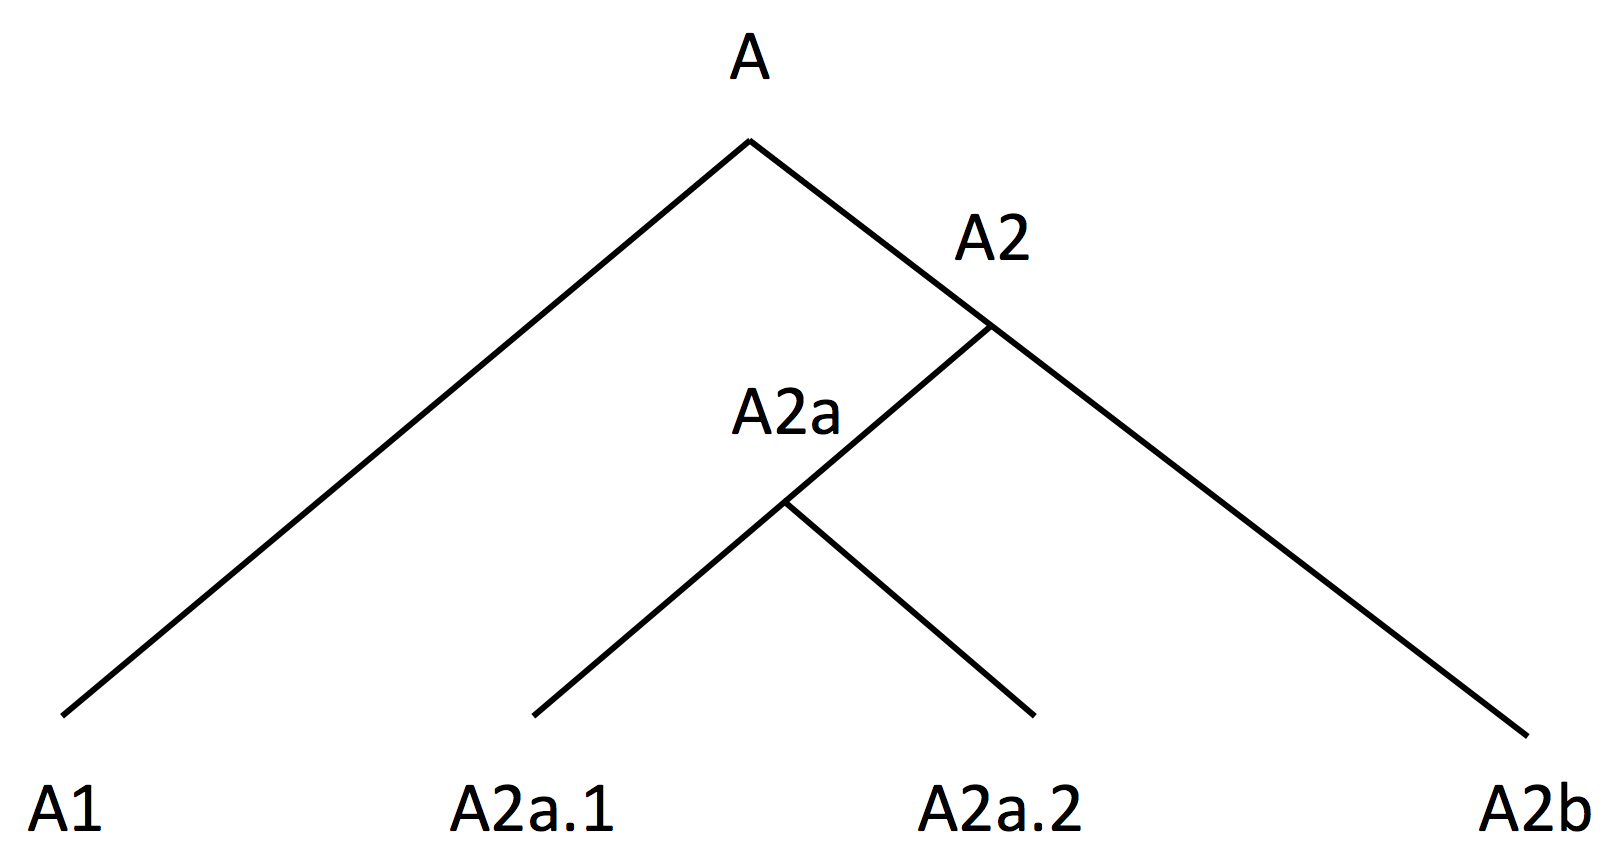
\includegraphics[width=0.60\textwidth,keepaspectratio]{figures/FigTree}
\caption{Tree diagram representing divergence by descent with modification. A1, A2a.1, A2a.2, and A2b are common descendants of A.}
\end{figure}

Diversification of languages, as in the history of great stocks like Bantu\is{Bantu language family}, Austronesian\is{Austronesian language family}, and Indo-European,\is{Indo-European language family} has long been represented with tree diagrams of this kind, in which the ostensible units of analysis are languages. By taking the language as the unit of analysis, tree diagrams must assume that languages cohere as units. Is this a fair assumption? Are language systems coherent, natural kinds? Or do we only imagine them to be? 

 

%Language history does show some causal biases toward vertical transmission, and our research needs to determine and account for the nature of these biases (see Chapter 4, below). But biases toward vertical transmission are significantly weaker than comparable biases in vertebrate lineages in biology. Historical processes in language differ in two fundamental ways from the kind of vertical transmission we see in the evolution of species in vertebrates. First, in addition to the vertical transmission that accounts for what is shared among daughter and parent languages, there is often extensive horizontal transmission, by which traits of a daughter language are neither inherited from a parent language nor internally innovated, but are adopted from a contact language. Nothing like this kind of horizontal transmission --- at least not on anything remotely like this scale --- occurs in the biological evolution of vertebrates. 

When tree diagrams are used to represent the history of diversification within a family of languages, there is an analogy with the kind of evolution\is{evolution!biological} seen in life forms that show a total or near-total bias toward vertical transmission in evolution, namely vertebrates\is{vertebrates} such as primates, birds, fish, and reptiles. So let us consider what the tree diagram means in the case of vertebrate natural history. Each binary branching in the tree represents a definitive split in a breeding population. The populations represented by daughter nodes inherit traits that were found in the parent population. Members of the daughter populations also commonly inherit modifications of the parent traits that significantly distinguish the two daughter populations from each other. Inheritance happens in events of sexual reproduction, in which complete genotypes are bestowed in the conception of new individuals. This encapsulation of the genome in causal events of inheritance ensures the vertical transmission that a tree diagram represents so well. In vertebrate species, when two populations are no longer able to interbreed, they can no longer contribute to each other's historical gene pool. This would be \textit{horizontal transmission},\is{horizontal transmission} something that is essentially absent from vertebrate evolution (though with some caveats; \citealt{koonin_darwinian_2009}). The tree representation is adequate in the case of vertebrate speciation\is{speciation} for one reason: the tree diagram does not capture horizontal transmission. The vertebrate genome\is{genetics} is essentially acquired by the individual organism as a bundle. So the complete organism can reasonably be treated as a unit for describing transmission and change in phylogeny\is{phylogenetic frame}. The vehicle for replication is the individual organism as defined by the structurally coherent entity that we call the body.

The problem is that while vertebrates have been implicitly taken to be the model for language, they are not like language in causal terms. They are not even representative of life forms\is{life forms} in general. Most forms of life, including not only the non-animal Eukaryotes, but also the Bacteria and Archaea, are not subject to strong vertical transmission\is{vertical transmission} constraints \citep{boto_horizontal_2010}. Most forms of life lack the bounded body plans that delineate vehicles or interactors for passing on replicable traits. The overall phenotypic structures of \textquoteleft individuals' in many species are to a large degree emergent. Evolutionary\is{evolution!biological} processes can be more clearly seen to operate on \textit{parts} of organisms \citep{dawkins_selfish_1976}.



\section{Linguistic systems}


People find it easy to accept \textquoteleft the language'\is{languages, as unit of analysis} as a unit of causal analysis. Our intuitions suggest that languages are effectively bounded, whole systems. We readily think of them as organisms. But they can also be thought of as focussed bundles of items. Indeed they should be thought of in this way, for the \textquoteleft linguistic system' is not a natural kind. 

The point has been made for linguistic systems with most clarity and rigor by \citet{le_page_acts_1985}. A prerequisite to the idea of a language (e.g. English) is the idea of a group of people who speak it. But as Le Page and Tabouret-Keller (\citeyear{le_page_acts_1985}) put it: 

\begin{quotation} Groups or communities and the linguistic attributes of such groups have no existential locus other than in the minds of individuals. (p. 4) We do not ourselves then need to put a boundary around any group of speakers and say \textquoteleft These are the speakers of Language A, different from Language B', except to the extent that the people think of themselves in that way, and identify with or distance themselves from others by their behaviour. (p. 9)
\end{quotation}

The point was made a half-century ago for social systems more generally by the anthropologist Edmund \citet{leach_political_1964}, in critiquing the structuralism of Radcliffe-Brown and students \citep{fortes_african_1940}: 

\begin{quotation}
Social systems were spoken of as if they were naturally existing real entities and the equilibrium inherent in such systems was intrinsic. (p. x)  I do not consider that social systems are a natural reality. In my view, the facts of ethnography and of history  can only \textit{appear} to be ordered in a systematic way if we impose upon these facts a figment of thought. (p. xii) 
\end{quotation}

Fair enough. But there must be some natural reality upon which we may impose our figments of thought. One candidate is the economy of \textit{bits} of language or culture, each of which has mobility: the words and other things that we can borrow from outside, without having to borrow the whole systems they come from. As \citet[22]{hudson_sociolinguistics_1996} puts it:

\begin{quotation}
We need to distance ourselves somewhat from the concepts represented by the words \textit{language} and \textit{dialect}, which are a reasonable reflection of our lay culture, called \textquoteleft common-sense knowledge', but not helpful in sociolinguistics. First, we need a term for the individual \textquoteleft bits of language' to which some sociolinguistic statements need to refer, where more global statements are not possible.
\end{quotation}

Hudson introduces \textit{linguistic item}\is{linguistic item} as a term for this unit with causal reality. Suppose that items --- in bundles --- are what we impose an essence upon when we imagine languages. Our vernacular language names would be labels for these imposed, imagined essences.\footnote{If the reader is concerned that the true holistic system nature of languages is being underestimated, see Chapter \ref{itemsystemproblem}, below.}


\section{Linguistic items}

The idea that languages are causally real units\is{languages, as unit of analysis} gets weaker when we think of the mechanisms of language transmission, both across and within generations. There are two problems for the language-as-real-system idea. First is that causal processes of transmission can be observed most concretely operating upon items\is{linguistic items} (e.g., in the borrowing and learning of words), not on whole systems. The second is that horizontal transmission\is{horizontal transmission} occurs. All parts of a language appear in principle to be independently mobile (though of course some bits of language travel more freely than others; \citealt{thomason_language_1988,curnow_what_2001,thomason_language_2001}). Now consider these points more closely.

What is transmitted in language history? It is not the whole system at once, but the components of the system, piece by piece and chunk by chunk, in millions of distinct events. Never all at once but at separate moments, over days, weeks, months and years. To be sure, the result of language transmission is a high degree of overlap among idiolects\is{idiolects} in a human population.\footnote{On idiolect overlap or convergence, cf. \citet{bakhtin_dialogic_1981}, \citet[106-7, 157-8]{hockett_refurbishing_1987}, \citet[227-8]{lee_whorf_1996}.} The overlap is so high that our idiolects are practically indistinguishable. And this reassures us that systems are real wholes. How does this degree of idiolect overlap come about? 

Part of the answer is that speech communities\is{speech community} are inward-focused. People in a group transmit linguistic items when they converse and interact. This creates an economy of signs, in the sense of \citet{zipf_human_1949}. When people in a group interact repeatedly, more signs come to be shared among those people. And the more that signs are shared, the more readily those people interact. This feedback effect in the social circulation of linguistic items is both a result of, and a cause of, common ground\is{common ground} in a community. People have more common ground because they interact more; they interact more because they have more common ground. The basic causal units, though, are the shared items, not the systems that emerge.

The second problem with `the language' as a natural unit is the ease of borrowing\is{borrowing} linguistic items. Languages constantly incorporate new structures, and quickly. When confronted with this kind of horizontal transmission, students of language change have looked for ways to distinguish it from a vertical\is{vertical transmission} signal, usually to then exclude it. But if horizontal transmission\is{horizontal transmission} is so widespread, this should cause people to doubt the value of a model in which vertical transmission is the main object of interest for representing and understanding language history. With a proper understanding of the causality of language change, we see that tree diagrams\is{tree diagrams} that take \textquoteleft the language' as the unit of analysis not only abstract from reality, they distort it. They are poor conceptual tools for understanding the ontology of language.\is{ontology of language} The solution is to change our assumptions about the causal units involved.

For Darwinian\is{Darwin} evolution\is{evolution} to occur, there must be a population of essentially equivalent but non-identical units. These units must inherit traits from comparable units that existed prior to them. And these inheritable traits must show variation that can result in comparable units having different chances of surviving to pass on those traits to a new generation. What are the units? In the case of vertebrates, a received view is that two sorts of units work together: organisms, and genes. Organisms are vehicles for replicating genes\is{genetics}. In vertebrates\is{vertebrates}, the vehicles for inheritance of traits are the bodies of individuals. Each body is a phenotypic instantiation of the system. But here is the problem. The situation with languages is not like this at all. 


\section{Thinking causally about language change}
We want a causal account of languages as historically evolved systems. To think concretely about this, consider the following. All the conventional bits of language you learned as an infant\is{first language acquisition} were created by enormous chains of social interaction in the history of a population. Each link in the chain was an observable instance of usage, a micro-scale cycle of transmission, going from public (someone uses a structure when speaking) to private (a second person's mental state is affected when the structure is learnt or entrenched) and back to public (the second person uses the structure, exposing someone else), and so on. This may seem to be an overly micro-perspective way of putting it. But it is important to be explicit about the proximal mechanisms of transmission. Causal statements about language often highlight only a part of what is going on. 

Consider (1) and (2):


\begin{enumerate}
\item \textit{Knowledge of grammar causes instances of speaking.} 
\item \textit{Instances of speaking cause knowledge of grammar. }
\end{enumerate} 

Statement (1) focuses on competence\is{competence}. It points to mechanisms of, and prerequisites for, saying things. Statement (2) focuses on performance\is{performance} and emphasizes its outcomes. We learn about language from what people say. But there is no contradiction between the statements shown in (1) and (2). They are ways of framing the same thing. Competence and performance are equally indispensable in the processes of historical evolution that determine and constrain what a language can be like. Words are effectively competing for our selection\is{selection} \citep{croft_explaining_2000}. If all goes well, we select the items that best enable us to manipulate other people's attentional and interpretive resources \citep[16-17]{enfield_relationship_2013}. 

\section{The problem with tree diagrams}

Tree diagrams\is{tree diagrams} of language diversification are good for some things, but they are not good for representing causal processes of language history, nor the natural, causal ontology of languages and language relatedness.\is{ontology of language} The tree diagram assumes that we are primarily interested in one form of transmission of heritable characteristics, namely, vertical transmission\is{vertical transmission} of features from a parent to a daughter language, normally through first language acquisition\is{first language acquisition} in children. The alternative --- horizontal transmission\is{horizontal transmission}, i.e., transmission of features between languages whose speakers are in contact, normally involving adult language learning --- is acknowledged but is regarded as noise that needs to be factored out from the vertical historical signal of primary interest (though note that some recent work applying new methods is showing promising signs of a shift in direction here; e.g., \citealt{reesink_explaining_2009}).

The tree diagram is a methodological simplification. It requires us to abstract from the causal facts. Of course this abstraction may be a harmless practical necessity. But our question is whether the abstraction inherent in the tree diagram does \textit{conceptual} harm. I think the answer is yes. It directs our attention away from the causal mechanisms that define language as an evolutionary process, and languages as evolved systems.

To begin to think causally we first need to explore the multiple frames within which causal processes may be effected. This is the topic of the next chapter. 

%\begin{list}{label}{spacing}
%\item (a) 	being exposed to semiotic material by which they may infer the idea; 

%(b) 	being motivated to infer the idea, and to actually create a representation of the idea; 

%(c) 	identifying as a person who would put the idea into practice;

%(d) 	putting the idea into practice, exposing others (back to (a)). 

%\end{list}





%If it is the material restrictions of time, space, social group size and the need for convention that create the very high levels of convergence in the linguistic behaviour and complex sign systems of social associates, then what accounts for the �system properties� of language, such as Greenbergian implicational universals? \textit{(The same question may be asked in anthropology generally, but linguistic anthropology allows us greater control.)} 


%Mead (1934:133) said �The processes of experience which the human brain makes possible are made possible only for a group of interacting individuals: only for individual organisms which are members of a society; not for the individual organism in isolation from other individual organisms�. (quoted in Rogoff 1990:14). See also Rosaldo (1984:145) for refs to Halliwell, Mead, Mauss and Fortes.

%Seeing that it is now widespread, we assume it has spread widely. This implies a time depth for the spreading process, as well as a source and direction of the spread. There is evidence of a process which may be described as epidemiology (Sperber 1985). People catch ideas for ways of saying things. Factors familiar to us from the field of sociolinguistics have licensed and constrained the transmission and adoption of new ways of saying things from one group of people to another. The current synchronic state is the outcome of such a process.

%The durability of signs is only maintained through constant field-testing of one's personal hypotheses about linguistic meaning. When you ask for \textit{salt} and get salt rather than pepper, your theory of the sign-category association <salt> is tested, confirmed, and therefore not revised. (There is no qualitative distinction, in this respect, between individual theories of the meanings of particular words, on the one hand, and grammatical categories, on the other.)


%\textit{The study of areal phenomena both force us to consider, and help us to answer, the central question of linguistics: What is the nature of language? What is the ontology of language?}




\chapter{Causal frames}
\label{causaldynamics}



If you really want to understand language, you will have to study a lot of different things. Here are some:

\begin{enumerate}
\item[\textbullet] {The finely-timed perceptual, cognitive, and motoric processes involved in producing and comprehending language}\is{processing}
\item[\textbullet] {The early lifespan processes by which children learn linguistic and communicative knowledge and skills}\is{first language acquisition}
\item[\textbullet] {The evolutionary\is{evolution!biological} processes that led to the unique emergence of the cognitive capacities for language in our species}
\item[\textbullet] {The ways in which the things we say are moves in sequences of social actions}\is{social action}
\item[\textbullet] {The mechanisms and products of language change, with links between historical processes and evolutionary processes}\is{language change}\is{evolution!historical}
\item[\textbullet] {Linguistic variation\is{variation} and its role in how historical change in language takes place in human populations}
\item[\textbullet] {Things that can be described without reference to process or causation at all, as seen in linguistic grammars,\is{grammars} dictionaries\is{dictionaries}, ethnographies\is{ethnographies}, and typologies\is{typologies}, where relationships rather than processes are the focus}
\end{enumerate}
%\footnote{On language production and comprehension, see for example Levelt 1989, 2012; Emmorey 2002; McNeill 2005; Cutler 2012. On language acquisition see Brown and  Gaskins, 2014; Schieffelin and Ochs 1986; Tomasello 2003. On language evolution see Hurford 2007, 2012;  Tomasello 2008; Hauser, Chomsky, and Fitch 2002; Chomsky 2011. On conversational sequence, see Schegloff 1968; Goffman  1981a; Goodwin 2000, 2006; Sidnell and Stivers 2012; Enfield 2013;  Enfield and Sidnell 2014; Sidnell and Enfield 2014. On language change, see Dixon  1997; Harris and Campbell 1995; Hopper and Traugott 1993; Hanks 2010; for evolutionary perspectives, see Boyd and Richerson 1985, 2005; Durham 1991; Smith, Brighton, and Kirby 2003; for the role of variation in change, see Labov 2011;  Trudgill 2010; Eckert 2000.}

These different points of focus correspond roughly with distinct research 
perspectives. But they do not merely represent disciplinary 
alternatives. The different perspectives can be seen to 
fit together as parts of a larger conceptual framework. 



To give some outline to that framework, I here define six interconnected frames for orienting our work. They remind us of the 
perspectives that are always available and potentially relevant, but that we might 
not be focusing on. They do not constitute a definitive set of 
frames -- there is no definitive set -- but they are useful. They correspond 
well to the most important causal domains.\is{causal frames} They conveniently group 
similar or tightly interconnected sets of causal mechanism under single 
rubrics. And together they cover most of what we need for providing 
answers to our questions in research on language. 


The frames are \textit{Microgenetic}, \textit{Ontogenetic}, 
\textit{Phylogenetic}, \textit{Enchronic}, \textit{Diachronic}, 
and \textit{Synchronic}. The meanings of these terms are explicated below. As a mnemonic, they spell MOPEDS\is{MOPEDS framework}. Frames like these are sometimes referred to as \textit{time scales}\is{time scales}. But calling them `scales' is not accurate. It implies that they all measure the same thing, just with arbitrarily different units of measure -- seconds versus minutes versus hours, etc. But the difference between, say, ontogenetic and diachronic (ditto for the other frames) is not defined in terms of abstract or objective units of the same underlying stuff -- time, in this case. The frames are defined and distinguished in 
terms of different types of underlying processes and 
causal-conditional mechanisms. For each frame, what 
matters most is how it works, not how long it takes. 



By offering a scheme of interrelated causal frames as part of a conceptual 
framework for research on language, I want to stress two points. 



The first is that these frames are most useful when we keep them 
conceptually distinct. Kinds of reasoning that apply within one frame do 
not necessarily apply in another, and data that are relevant in one 
frame might not be relevant (in the same ways) in another. Mixing up these frames leads to confusion. 



The second point is that for a full understanding of the 
things we study it is not enough just to understand these 
things from within all of the different frames. The ideal is also to 
show how each frame is linked to each other frame, and, ultimately, how 
together the frames reveal a system of causal forces 
that define linguistic reality.



\section{Distinct frames and forces}
\label{Distinctframesandforces}

The ethologist Niko Tinbergen famously emphasized that different kinds of research question may be 
posed within different theoretical and methodological frames, and may 
draw on different kinds of data and reasoning \citep{tinbergen_aims_1963}. See \tabref{tinbergenfour}.



\begin{table}[h]
\centering
\begin{tabular}{ll}
\lsptoprule
\textbf{Causal} & What is the mechanism by which the behavior occurs?
\\
%\hline
\textbf{Functional} & What is the survival or fitness value of the 
behavior? \\
%\hline
\textbf{Phylogenetic} & How did the behavior emerge in the course of 
evolution? \\
%\hline
\textbf{Ontogenetic} & How does the behavior emerge in an individual's 
lifetime? \\
\lspbottomrule
\end{tabular}
\caption{Distinct causal/temporal frames for studying animal 
behavior, after \citet{tinbergen_aims_1963}.}
\label{tinbergenfour}
\end{table}



Tinbergen's four questions were applied in studying the behavior of 
non human animals. The distinctions were designed to handle 
communication systems such as the mating behavior of stickleback fish\is{stickleback fish}, 
not the far greater complexities of language, nor the rich cultural 
contexts of language systems. If we are going to capture the spirit of 
Tinbergen's idea, we need a scheme that better covers the phenomena 
specific to language and its relation to human diversity\is{diversity}. 


Many researchers of language and culture have emphasized the need to monitor and distinguish different causal frames that determine our perspective. These include researchers of last century \citep{saussure_cours_1916,vygotsky_thought_1962} through 
to many of today \citep{tomasello_constructing_2003,macwhinney_emergence_2005,raczaszek-leonardi_multiple_2010,cole_phylogeny_2007,donald_slow_2007,larsen-freeman_complexity_2008,uryu_ecology_2014,lemke_across_2000,lemke_language_2002}. We now consider some of the distinctions they have offered.



The classical two-way distinction made by \citet{saussure_cours_1916} -- \textit{synchronic}\is{synchronic frame} versus \textit{diachronic}\is{diachronic frame} -- is the tip of the iceberg. In a synchronic frame, we view language as a static 
system of relations. In a diachronic frame, we look at the historical processes of change that give rise to the synchronic relations observed. But if you look at the dynamic nature of language you will quickly see that 
diachrony -- in the usual sense of the development and 
divergence of languages through social history -- is not the only dynamic frame. 



Vygotsky distinguished between \textit{phylogenetic}\is{phylogenetic frame}, \textit{ontogenetic}\is{ontogenetic frame}, and \textit{historical} processes, and stressed that 
these dynamic frames were distinct from each other yet interconnected. 
His insight has been echoed and developed, from 
psychologists of communication like \citet{tomasello_cultural_1999} and \citet{cole_phylogeny_2007} to computational linguists like \citet{steels_synthesizing_1998,steels_evolving_2003} and \citet{smith_complex_2003}. 



\citet[540]{smith_complex_2003} argue that to understand language we have to see it 
as emerging out of the interaction of multiple complex adaptive systems. They name three ``time scales''\is{time scales} that need to be taken into account -- \textit{phylogenetic}\is{phylogenetic frame}, \textit{ontogenetic}\is{ontogenetic frame}, and \textit{glossogenetic}\is{diachronic frame} 
(= ``cultural evolution'', i.e., diachronic) -- thus echoing 
Vygotsky. Language is, they write, ``a consequence of the interaction 
between biological evolution, learning and cultural evolution'' \citep[541]{smith_complex_2003}. R\k{a}czaszek-Leonardi focuses on psycholinguistic\is{psycholinguistics} research, and proposes that three frames need to be addressed: \textit{online}, \textit{ontogenetic} and \textit{diachronic}. She leaves out the phylogenetic frame, but adds the ``online'' frame 
of cognitive processing\is{processing}. \citet[185]{cole_cultural_1996} expands the list of dynamic frames to include \textit{microgenesis}, \textit{ontogeny} (distinguishing early learning from 
overall lifespan), \textit{cultural history}, \textit{phylogeny}, 
and even \textit{geological time}. \citet[193--195]{macwhinney_emergence_2005} offers a list of ``seven markedly different 
time frames for emergent processes and structure'', citing Tinbergen's 
mentor Konrad \citet{lorenz_evolution_1958}. MacWhinney's frames are \textit{phylogenetic}, \textit{epigenetic}, \textit{developmental}, 
\textit{processing}, \textit{social}, \textit{interactional}, 
and \textit{diachronic}. 



\citet[122]{newell_unified_1990} proposes a somewhat more mechanical division of time 
into distinct ``bands of cognition'' (each consisting of three ``scales''). Newell takes the abstract/objective temporal unit of the second as a key 
unit, and defines each timescale\is{time scales} on a gradient from 10$^{-4}$ 
seconds at the fast end to 10$^{7}$ seconds at the slow end: the 
\textit{biological band} (= 10$^{-4}$-10$^{-2}$ seconds), the 
\textit{cognitive band} (= 10$^{-1}$-10$^{1}$ seconds), the 
\textit{rational band} (= 10$^{2}$-10$^{4}$ seconds), and the 
\textit{social band} (= 10$^{5}$-10$^{7}$ seconds). He also 
adds two ``speculative higher bands'': the \textit{historical band} (= 
10$^{8}$-10$^{10}$ seconds), and the \textit{evolutionary band} 
(= 10$^{11}$-10$^{13}$ seconds; \citealt[152]{newell_unified_1990}), thus suggesting a 
total of 18 distinct timescales. 



Like Newell (though without reference to him), \citet[277]{lemke_across_2000} takes 
the second as his unit and proposes no less than 24 ``representative 
timescales'',\is{time scales} beginning with 10$^{-5}$ seconds -- at which a typical 
process would be ``chemical synthesis'' -- through to 10$^{18}$ 
seconds -- the scale of ``cosmological processes''. 



Lemke's discussion is full of insights. But he generates his taxonomy by arbitrarily carving up an abstract gradient. It is not established in terms of research-relevant qualitative distinctions or 
methodological utility, nor is it derived from a theory (cf.  
Uryu et al \citeyear{uryu_ecology_2014}, \citeyear[169]{larsen-freeman_complexity_2008}). It is not clear, for example, why a distinction between units of 3.2 years 
versus 32 years should necessarily correlate with a distinction between 
processes like institutional planning versus identity change; nor why 
the process of evolutionary change should span three timescales (3.2 
million years, 32 million years and 317 million years) or why it should 
not apply at other timescales. 



\citet[169]{larsen-freeman_complexity_2008} propose a set of ``timescales\is{time scales} 
relevant to face-to-face conversation between two people'': a \textit{mental processing }timescale of milliseconds, a \textit{microgenetic }
timescale of online talk, a \textit{discourse event} timescale, a 
\textit{series of connected discourse events}, an \textit{ontogenetic }scale of an individual's life, and a \textit{phylogenetic} timescale. \citet{uryu_ecology_2014} critique this model for not explaining why these 
timescales are the salient or relevant ones, and for not specifying 
which other timescales are ``real but irrelevant''. 



\citet{uryu_ecology_2014} propose a principled ``continuum'' of timescales\is{time scales} running from 
``fast'' to ``slow'' (11 distinctions in the order \textit{atomic}, 
\textit{metabolic}, \textit{emotional}, \textit{autobiographical}, \textit{interbodily}, \textit{microsocial}, \textit{event}, 
\textit{social systems}, \textit{cultural}, \textit{evolutionary}, \textit{galactic}) that are orthogonal to a set of ``temporal 
ranges'' running from ``simple'' to ``complex'' (six distinctions in the 
order \textit{physical universe}, \textit{organic life forms}, 
\textit{human species}, \textit{human phenotype}, \textit{
dialogical system}, \textit{awareness}). Uryu et al's approach 
applies the notion of ecology to the dynamics of language and its usage (see also \citealt{cowley_distributed_2011}, \citealt{steffenson_ecolinguistics:_2013}).



What to make of this array of multi-scale schemes? Some are well-motivated but incomplete. Saussure gives 
a single dynamic frame, leading us to wonder, for example, whether we 
should regard speech processing as nano-diachrony\is{nano-diachrony}. Vygotsky gives us three dynamic frames, but does not single out or 
sub-distinguish ``faster'' frames like microgeny\is{microgenetic frame} and enchrony\is{enchronic frame}. Are we to 
think of these as pico-ontogeny?\is{pico-ontogeny} On the other hand, some schemes give us 
finer differentiation than we need, or offer arbitrary 
motivations for the distinctions made. What we need is a middle way. 



\section{MOPEDS: A basic-level set of causal frames}
\is{MOPEDS framework}

Of the frames discussed in the previous section, six capture 
what is most useful about previous proposals. These six frames are relatively well understood. They are known to be 
relevant to research. They are well-grounded in prior work on language and 
culture. And they are known to be related to each other in interesting ways.\footnote{One might wonder if one or more of these frames might be reduced in terms of one or more others. It is reminiscent of the idea of reducing social processes to physical ones: Were such a reduction possible, it is unlikely to be helpful.} This is what we need: a basic-level set of conceptually 
distinct but interconnected causal frames for understanding language. 



Each of the six frames -- microgenetic, ontogenetic, phylogenetic, 
enchronic, diachronic, synchronic -- is distinct from the others in terms 
of the kinds of causality it implies, and thus in its relevance to what 
we are asking about language and its relation to culture and other 
aspects of human diversity. One way to think about these distinct frames 
is that they are different sources of evidence for explaining the things 
that we want to understand. I now briefly define each of the six frames.



\subsection{Microgenetic (action processing)}
\is{microgenetic frame}


In a microgenetic frame, we look at how language and culture are psychologically processed. For example, in order to produce a simple sentence, a person goes through a set of 
cognitive processes including concept formulation, lemma retrieval, and phonological 
encoding \citep{levelt_speaking:_1989}. Or when we hear and understand what someone says \citep{cutler_native_2012}, we have to parse the 
speech stream, recognize distinct words and constructions, and infer 
others' communicative intentions. 

These processes tend to take place at time scales between a few 
milliseconds and a few seconds. Causal mechanisms at this 
level include working memory \citep{baddeley_working_1986}, rational 
heuristics \citep{gigerenzer_heuristics:_2011}, minimization of
effort \citep{zipf_human_1949}, categorization, motor routines, 
inference, ascription of mental states such as beliefs, 
desires, and intentions \citep{searle_intentionality:_1983,enfield_roots_2006}, and 
the fine timing of motor control and action execution.



\subsection{Ontogenetic (biography)}
\is{ontogenetic frame}


In an ontogenetic frame, we look at how a 
person's linguistic habits and abilities are learned and
developed during the course of that person's lifetime. Many of the 
things that are studied within this frame come under the general 
headings of language acquisition and socialization. This refers to both
the learning of a first language by infants\is{first language acquisition} (see \citealt{clark_first_2009}, \citealt{brown_language_2014}) and the learning of a second 
language by adults \citep{klein_second_1986}.\is{second language acquisition} 



The kinds of causal processes seen in the ontogenetic frame include strategies 
for learning and motivations for learning. Some of these strategies and 
motivations can be complementary, and some may be employed at distinct 
phases of life. Causal processes involved in this frame include 
conditioning, statistical learning and associated mechanisms like 
entrenchment and pre-emption \citep{tomasello_constructing_2003}, adaptive docility\is{docility} \citep{simon_mechanism_1990}, a pedagogical stance \citep{gergely_sylvias_2006}, and long-term 
memory \citep{kandel2009biology}.



\subsection{Phylogenetic (biological evolution)}
\is{phylogenetic frame}


In a phylogenetic frame we ask how our species first became able to learn and use language. This is part of a broader set of questions about the 
biological evolution and origin of humankind.\is{evolution!biological} It is a difficult topic to 
study, but this has not stopped a vibrant bunch of researchers from 
making progress \citep{hurford_origins_2007,hurford_origins_2012,levinson_language_2014}.\is{evolution!of language capacity} 



Causal processes in a phylogenetic frame include those typically described in evolutionary biology. They invoke 
concepts like survival, fitness, and reproduction of biological 
organisms \citep{ridley_evolution_1997,ridley_evolution_2004}, which in the case of language means 
members of our species. The basic elements of 
Darwinian natural selection\is{selection} are essential here: competition among individuals in a 
population, consequential variation in individual characteristics, 
heritability of those characteristics, exaptation, non-telic design, and so forth \citep{darwin_origin_1859,dawkins_selfish_1976,jacob_evolution_1977,mayr_growth_1982}.



\subsection{Enchronic (social interactional)}
\is{enchronic frame}


In an enchronic frame, we look at language in the context of social interaction.\is{social interaction} When we communicate, we use sequences of moves made up of speech, gesture,\is{gesture} and other kinds of signs. The causal processes of interest involve structural relations of sequence 
organization (practices of turn-taking and repair which organize our 
interactions; \citealt{schegloff_sequencing_1968,schegloff_sequence_2007,sacks_simplest_1974,schegloff_preference_1977,sidnell_handbook_2012}) and ritual or affiliational relations of 
appropriateness, effectiveness, and social accountability \citep{heritage_garfinkel_1984,atkinson_structures_1984,stivers_morality_2011,enfield_relationship_2013}. 



Turn-taking\is{turn-taking} in conversation\is{conversation} operates in the enchronic 
frame, as do speech act\is{speech acts} sequences such as question-answer, 
request-compliance, assessment-agreement, and suchlike (see \citealt{enfield_language_2014}). Enchronic processes tend to take place at a temporal 
granularity around one second, ranging from fractions of seconds up to 
a few seconds and minutes (though as stressed here, time units are not 
the definitive measure; exchanges made using email or surface mail may stretch out over much greater lengths of time). 



Enchronic processes and structures are the focus in 
conversation analysis and other traditions of research on communicative 
interaction. Some key causal elements in this frame include relevance \citep{garfinkel_studies_1967,grice_logic_1975,dan_sperber_relevance:_1995}, local motives \citep{schutz_phenomenology_1970,leontev_problems_1981,heritage_garfinkel_1984}, sign-interpretant relations (\citealt{kockelman_semiotic_2005,kockelman_agent_2013}, \citealt[Chapter 4]{enfield_relationship_2013}), and social accountability \citep{garfinkel_studies_1967,heritage_garfinkel_1984}.



\subsection{Diachronic (social/cultural history)}
\is{diachronic frame}


In a diachronic frame, we look at elements of language as historically 
conventionalized patterns of knowledge and/or behavior. If the question 
is why a certain linguistic structure is the way it is, a diachronic 
frame looks for answers in processes that operate in historical 
communities. While of course language change has to be actuated\is{actuation} at a 
micro level \citep{weinreich_empirical_1968,labov_mechanism_1986,eckert_linguistic_2000}, for a linguistic item to be found in a language, that 
item has to have been diffused\is{diffusion} and adopted throughout a community 
before it can have become a convention. 



Among the causal processes of interest in a diachronic frame are the 
adoption and diffusion of innovations, and the demographic ecology that 
supports cultural transmission \citep{rogers_diffusion_2003}. Population-level 
transmission is modulated by microgenetic\is{microgenetic frame} processes of extension, inference, and reanalysis that feed grammaticalization\is{grammaticalization} 
\citep{hopper_grammaticalization_1993}. 



Of central importance in a diachronic frame are social processes of 
group fission and fusion \citep{aureli_fission-fusion_2008}, migration \citep{manning_migration_2005}, and sociopolitical relations through history \citep{smith_inquiry_1776,marx_german_1947,runciman_theory_2009}. The timescales of interest in a 
diachronic frame are often stated in terms of years, decades, and 
centuries.



\subsection{Synchronic (representation of relations)}
\is{synchronic frame}


Finally, a synchronic frame is different from the other frames mentioned 
so far because time is removed from consideration, or at least 
theoretically so. One might ask if it is a causal frame at all. But 
if we think of a synchronic system as a true description of the items 
and relations in a person's head, as coded, for example, in their 
memory, then this frame is real and relevant, with causal implications, 
even if we see it as an abstraction (e.g., as bracketing out 
near-invisible processes that take place in the fastest levels of 
Newell's ``biological band''; see section \ref{Distinctframesandforces}, above). 



In Saussure's famous comparison, language is like a game of chess. If we 
look at the state of the game half way, a diachronic\is{diachronic frame} frame 
would view the layout in terms of the moves that had been made up 
to that point, and that had created what we now see. A 
synchronic account would do no more than describe the positions and 
interrelations of the pieces on the board at that point in time. For an 
adequate synchronic description, one does not need to know how the set 
of relations came to be the way it is. 



There are two ways to take this. One is to see the synchronic frame as a purely 
methodological move, an abstraction that allows the professional 
linguist to describe a language as a whole system that hangs together. 
Another -- not in conflict with the first -- is to see the 
synchronic description of a language as a hypothesis about what is 
represented in the mind of somebody who knows the language. 



A synchronic system cannot be an entirely atemporal concept. At the very 
least this is because synchronic structures cannot be inferred without 
procedures that require time; e.g., the enchronic\is{enchronic frame} sequences that we use
in linguistic elicitation with native speaker informants. But a synchronic system is 
clearly distinct from an associated set of ontogenetic processes,\is{ontogenetic frame} on the one hand, 
and diachronic\is{diachronic frame} processes, on the other (though it is causally 
implied in both). We can infer an adult's knowledge of language and 
distinguish this from processes including the learning that led to this 
knowledge and the history that created the conventional model for 
this knowledge (but which neither the learner nor the competent speaker 
need have had access to). 



The goal here is to define frames that are relevant to a natural, causal account of language. So when I talk about a 
synchronic frame I mean a way of thinking about the conceptual representations of a language that make it possible for people to produce and interpret utterances in that language. 



Causality in a synchronic frame is tied to events that led \textit{to} 
the knowledge, and to events that may lead \textit{from} it, as well as how the 
nature and value of one convention may be dependent on the nature and 
value of other conventions that co-exist as elements of the same system.



\section{Interrelatedness of the frames}



How are these frames interrelated? As \citet[276]{raczaszek-leonardi_multiple_2010} says, ``even if a researcher aims to focus on a particular scale and system, he 
or she has to be aware of the fact that it is embedded in others''. Other 
authors (\citealt[179]{cole_cultural_1996}, \citealt[192]{macwhinney_emergence_2005}) have asked: What are the 
forces that cause these frames to ``interanimate'' or ``mesh''? The way to find out would be to test and extend the useful suggestions of authors like \citet{newell_unified_1990}, \citet[184--185]{cole_cultural_1996}, \citet{macwhinney_emergence_2005}, \citet[279--286]{lemke_across_2000} and \citet{uryu_ecology_2014}. 



How might the outputs of processes foregrounded within any one of these 
explanatory frames serve as inputs for processes foregrounded within any 
of the others? Answers to this question will greatly enrich our tools for 
explanation.



\section{The case of Zipf's length-frequency rule}
\label{zipflengthrule}
\is{length-frequency rule}
Why is it good to have a set of distinct causal frames for language?
Because it offers explanatory power. Consider the observation made by Zipf that ``every language shows an inverse relationship between the lengths 
and frequencies of usage of its words'' \citep[66]{zipf_human_1949}.\footnote{I am grateful to Martin Haspelmath for insisting on the distinction between Zipf's Law and Zipf's length-frequency rule (cf. \citealt{NewmanPowerLaws2006}). Zipf's Law states that there is a correlation between the frequency of an item and its frequency rank relative to other items in a set. His length-frequency rule states that the shorter a word is, the more frequently the word is used.} Zipf suggested that the correlation between word length and frequency is explained by a psychological preference for minimizing 
effort.\is{minimal effort principle} If we take this as a claim that synchronic structures in 
language are caused by something psychological -- though Zipf's own claims 
were rather more nuanced -- this raises a linkage problem\is{linkage problem} (\citealt[201]{clark_psychological_1984}). 



The problem is that a person's desire to minimize effort cannot directly affect a synchronic system's structure. 
A cognitive preference is a property of an individual, while a synchronic 
fact is shared throughout a population. Something must link the two. 
While it may be true that the relative length of the words I know 
correlates with the relative frequency of those words, this fact was 
already true of my language before I was born. The correlation cannot have been caused by my cognitive 
preferences. How, then, can the idea be explicated in causal terms?



As was clear to \citet{zipf_human_1949}, to solve this problem we appeal to 
multiple causal frames.\is{causal frames} We can begin by bringing diachronic\is{diachronic frame} processes 
into our reasoning. A presumption behind an account like Zipf's is 
that all members of a population have effectively the same biases.\is{cognitive biases} The key to understanding the status of a microgenetic\is{microgenetic frame} bias like 
``minimize effort in processing where possible'' is to realize that this 
cognitive tendency has an effect only in its role as a \textit{transmission bias}\is{transmission biases} in a diachronic process of diffusion\is{diffusion} of convention 
in a historical population (see below chapters for explication of 
diachrony as an epidemiological\is{epidemiology} process of biased transmission, 
following Rogers \citeyear{rogers_diffusion_2003}, Sperber \citeyear{sperber_anthropology_1985}, and Boyd and Richerson \citeyear{boyd_culture_1985,boyd_origin_2005}). The synchronic\is{synchronic frame} facts are an aggregate outcome of individual people's biases multiplied in a community and through time. The bias has a 
causal effect precisely in so far as it affects the likelihood that a
pattern will spread throughout that community. 



Now, while the spread of a pattern and its maintenance as a convention in a group are diachronic\is{diachronic frame} processes, a transmission bias can operate in three other frames. In an ontogenetic frame,\is{ontogenetic frame} a correlation between the shortness of words and the frequency of words might make the system easier to learn. This bias causes the correlation to become more widely distributed in the population. In a microgenetic frame,\is{microgenetic frame} people may want to save energy by shortening a word that they say often, again broadening the distribution of the correlation. And an enchronic frame\is{enchronic frame} will capture the fact that communicative behavior is not only regimented by individual-centered biases in learning, processing, and action, but also by the need to be successfully understood by another person if one's communicative action is going to have its desired effect. The presence of another person, who displays their understanding, or failure thereof, in a next move -- criterial to the enchronic frame -- provides a selectional counter-pressure against people's tendency to minimize effort\is{minimal effort principle} in communicative behavior. One's action has to be recognized by another person if that action\is{social action} is going to succeed (\citealt[21]{zipf_human_1949}, \citealt[Chapter 9]{enfield_relationship_2013}).



If we adopt a rich notion of a diachronic frame in which transmission 
biases play a central causal role, we can incorporate the ontogenetic, 
microgenetic and enchronic frames in explaining synchronic facts. We do this by invoking the mechanisms of \textit{guided variation}\is{guided variation} explicated by 
\citet{boyd_culture_1985,boyd_origin_2005} and explored in subsequent work by 
others \citep{kirby_function_1999,kirby_ug_2004,christiansen_language_2008,chater_language_2010}. This allows us to hold 
onto Zipf's insight, along with similar claims by authors such as 
Sapir before him, and Greenberg after him, who both also saw connections 
between individual-level psychological biases\is{cognitive biases} and community-level synchronic facts. \citet{greenberg_universals_1966} implied, for example, that there is a kind of cognitive 
harmony in having analogous structures in different parts of a language 
system. \citet[154--158]{sapir_language:_1921} suggested that change in linguistic 
systems by drift\is{drift} can cause imbalances and ``psychological 
shakiness'', which motivates the reorganization of grammar to avoid 
that mental discomfort. 



Similar ideas can be found in work on grammaticalization\is{grammaticalization} \citep{givon_syntax:_1984,bybee_language_2010} and language change\is{language change} due to social contact\is{language contact} \citep{weinreich_languages_1953}, leading to the same conclusion: Synchronic patterns can have 
psychological explanations but only when mediated by the aggregating 
force of diachronic processes.\is{diachronic frame} 



The point is central to explaining other observed 
correlations in language and its usage, for example that more frequent words change more slowly 
\citep{pagel_frequency_2007}, that differences in processes of 
attention and reasoning correlate with differences in the grammar of the 
language one speaks \citep{whorf_language_1956,lucy_language_1992,slobin_thought_1996}, 
that ways of responding in conversation\is{conversation} can be constrained by collateral 
effects\is{collateral 
effects} of language-specific grammatical structures \citep{sidnell_language_2012}, that tendencies in natural meaning\is{natural meaning} can correlate with universals\is{universals} in the sounds of words \citep{dingemanse_is_2013}, and that cultural values\is{cultural values} can shape grammatical categories \citep{hale_notes_1986,wierzbicka_semantics_1992,chafe_loci_2000,enfield_ethnosyntax:_2002,everett_cultural_2005,everett_language:_2012}. But most if not all of these claims bracket out some elements of the full 
causal chain involved. To give a complete and explicit account, multiple frames are needed.





 \newpage

\chapter{Transmission biases}
\label{Transmission biases}



Anyone who wants a natural, causal account of linguistic and other cultural transmission will have to study transmission biases.\is{transmission biases} These are the biases that ultimately regulate the historical, cumulative transmission of culture. To understand how the linguistic habits of communities change over generations --- in a diachronic frame\is{diachronic frame} --- we must also look in the ontogenetic frame,\is{ontogenetic frame} that is, in the process of language acquisition,\is{first language acquisition} and the resultant slight differences in habits of speech between generations. Language acquisition involves the effective transmission of a language from parents to children. Imperfections in this transmission are sometimes thought to explain language change.\is{language change} Consistent patterns in the details of such changes have been documented across a wide range of the world's languages. Many to argue that natural paths of semantic change are motivated by species-wide innate conceptual structure. There are universals\is{universals} in semantic change,\is{semantic change} independent from social factors and other factors outside the minds and bodies of speakers. But this is only part of the story. Even when new ideas for ways of saying things have their source within a single person, the spread of that idea follows mechanisms of population-level social transmission. And the success or failure of such transmission is ultimately dependent on the biases that are the topic of this chapter.

Cultural transmission can be usefully understood in relation to epidemiology\is{epidemiology} \citep{sperber_anthropology_1985}. We catch ideas from others, in this case ideas for attributing meanings to signs.


\begin{quotation}
	An innovation\is{innovation} in a language begins its existence in the mouths and minds of one or more speakers and spreads from them to other speakers. In fact, innovations occur constantly in the speech of individuals, but an innovation becomes part of the history of the language only when it spreads through the network to become a stable feature in the speech of a group of speakers. \citep[214-5]{ross_social_1997} 

\end{quotation}
	
	On syntax specifically, Harris and Campbell make a similar point:

\begin{quotation}
	Isolated creative, exploratory expressions are made constantly by speakers of all ages. Such expressions may be developed for emphasis, for stylistic or pragmatic reasons (to facilitate communication as in changes to avoid ambiguity or to foster easier identification of discourse roles), or they may result from production errors. The vast majority of such expressions are never repeated, but a few \textquoteleft catch on'. \citep[54]{harris_historical_1995}
\end{quotation}

\textit{How} do they catch on? How do they make this leap from single speaker to population-wide? How does an innovation become a stable feature in the speech of a group of speakers? In this chapter I discuss a crucial part of the answer to this question: the \textit{biases} that operate in linguistic and cultural change, in the diachronic frame.\is{diachronic frame} I will define some important biases, and I will say why we need a coherent conceptual framework to explain just why we observe the biases we observe. 


\section{Cultural epidemiology}
\is{epidemiology}

In the cultural evolution of language, that is, the diffusion, 
maintenance, and change of linguistic practices in historical 
communities, it is often assumed or implied that the unit of analysis is 
the language system as a whole.\is{languages, as unit of analysis} But the diachronic\is{diachronic frame} replication and transmission of 
whole language systems is not causally conducted directly at the system level (see Chapter \ref{causalunits} above). It 
is an aggregate outcome of a massive set of much simpler and much 
smaller concrete speech events that operate, in enchronic and microgenetic frames,\is{microgenetic frame} on the \textit{parts} of a language, such as words or pieces of grammar\is{linguistic items} 
\citep{hudson_sociolinguistics_1996}. 



Language systems only exist because populations of linguistic items 
replicate and circulate in human communities, whenever people say things. A causal account of language evolution\is{evolution!of languages} that focuses on the transmission of linguistic items can be called an 
epidemiological view, following \citet{sperber_anthropology_1985,sperber_explaining_1996}, 
and in a similar spirit to \citet{keller_language_1994} and \citet{croft_explaining_2000}. In an 
item-based account, the pieces of a system 
can change independently from other pieces, and they can be plucked out 
and borrowed from one system to another. This happens for example when we borrow a 
word. In diachronic\is{diachronic frame} processes, both enchronic\is{enchronic frame} and microgenetic\is{microgenetic frame} processes play a role.



Ultimately we need a causal account for why it sometimes seems like we 
can treat languages as if they were organism-like systems (e.g., when we 
write grammars). This is the topic of Chapter \ref{itemsystemproblem}, below. But first we need to define the basic underlying causal anatomy of item-based 
language transmission. Here I outline the basics of a transmission 
biases\is{transmission biases} approach to the historical evolution of languages. 



\section{Biased transmission}


The diffusion of cultural items in the diachronic frame\is{diachronic frame} is explained in terms of a \textit{biased transmission} model of the distribution of cultural knowledge 
and practice within human populations and across generations, following 
a general framework of cultural epidemiology\is{epidemiology} \citep{sperber_anthropology_1985,sperber_explaining_1996,boyd_culture_1985,boyd_origin_2005,enfield_linguistic_2003,enfield_transmission_2008}. In a biased transmission model, the question of whether 
fashions of cultural practice in a population spread, decline, 
transform, or remain as they are will be determined the cumulative 
effect of biases: filters, pumps, and transformers 
on cultural practices in a competition for social uptake. The processes are visible in the diachronic frame,\is{diachronic frame} but their proximal causal bases are seen in enchronic\is{enchronic frame} and microgenetic frames.\is{microgenetic frame}



Linguistic and other cultural items are not confined to the mind. Nor are they confined to things or actions that can be perceived. They are simultaneously manifest in mental \textit{and} 
material domains, \textit{and} in relations between these domains. At 
any moment, a community is buzzing with enchronic and microgenetic causal chains that constitute continuous lines of 
production and comprehension of pieces of language and culture. I am 
referring to people's courses of goal-directed action using words, tools, body movements, 
and other cultural items. 



These courses of behaviour are contexts in which the natural 
histories of cultural and linguistic items are played out. They 
constitute causal chains with links from mind (I know a word, I 
understand a tool) to usage (I use the word in conversation, I 
use the tool for a purpose), to mind (the other person learns or recognizes 
the word, an onlooker learns or recognizes the tool's 
function, attributing a goal to my behaviour), to usage, to mind, to 
usage, to mind, to usage, and so on. This type of causal 
trajectory is a chain of \textit{iterated practice},\is{iterated practice} or a cognitive 
causal chain\is{cognitive 
causal chain} \citep{sperber_why_2006-1}. See Figure \ref{iteratedpractice} for a simplified illustration.





\begin{figure}[h]
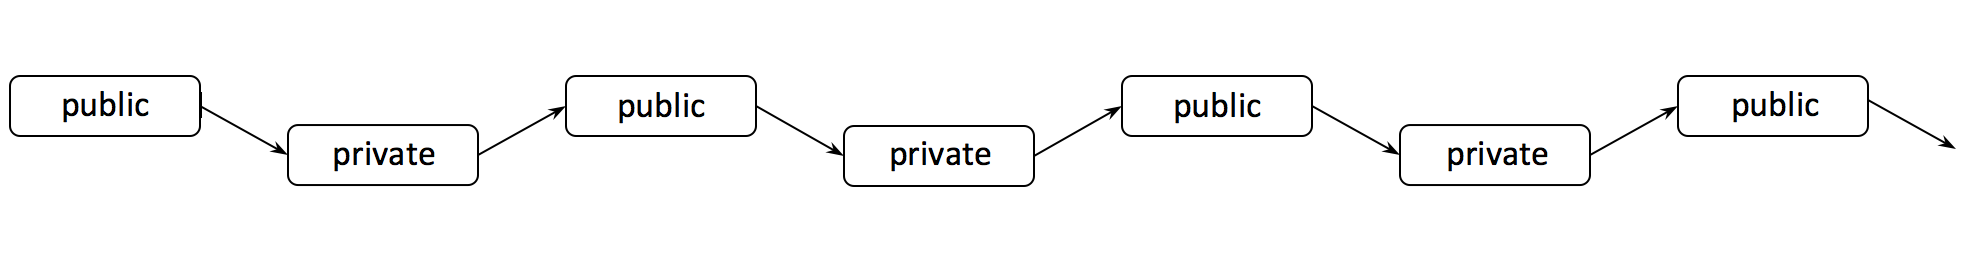
\includegraphics[width=0.95\textwidth,keepaspectratio]{figures/ch02fig01}
\caption{Simplified illustration of iterated practice, or a social 
cognitive causal chain (Sperber 2006:438).}
\label{iteratedpractice}
\end{figure}



Figure \ref{iteratedpractice} is not an \textit{iterated learning} chain,\is{iterated learning} of the kind presented by 
Kirby and colleagues \citep{kirby_ug_2004,kirby_cumulative_2008}, among 
others (\citealt{christiansen_language_2008}; see below). Those iterated learning depictions resemble Figure \ref{iteratedpractice}, 
but they are not the same. In iterated learning (studied to date using small, artificial languages in lab settings), each arrow from public 
to private may represent an entire learning process in an ontogenetic frame,\is{ontogenetic frame} such as a child's 
learning of a language.\is{first language acquisition} Each link in the chain is effectively a single 
macro-level state change in ontogeny (e.g., the move from not knowing 
the language to knowing the language). This is shorthand for a huge set 
of small events and small associated state changes. 



Learning a language involves not one event but many iterations of 
exposure and reproduction. In each micro-occasion of exposure and 
reproduction there is feedback that comes from others' reactions to how we use words in context. This feedback\is{feedback} plays 
an essential role in learning. Both the microgenetic\is{microgenetic frame} and ontogenetic frames\is{ontogenetic frame} are relevant. The iterated learning\is{iterated learning} model abstracts 
away from these details (not without practical reason), while the 
iterated practice\is{iterated practice} model in Figure \ref{iteratedpractice} tries to capture them directly and 
explicitly. 



While iterated learning focuses on the ontogenetic\is{ontogenetic frame} or biographical 
frame, iterated practice focuses on the enchronic 
frame,\is{enchronic 
frame} that is, the frame of moves and counter-moves in 
human interaction\is{social interaction} (see \citealt[10]{enfield_anatomy_2009}, \citeyear[Chapter 4]{enfield_relationship_2013}). In \ref{iteratedpractice}, each link in the chain from 
private-public-private does not represent a generation of individuals in 
a human population (by contrast with the comparable figure in 
\citealt{christiansen_language_2008}). It represents a generation of individuals 
in a population of items,\is{linguistic items} that is, one local cycle of 
instantiation of a practice, such as a single use of a word, a single 
performance of a ritual, or a single occasion of making bacon and eggs 
for breakfast. 



The schema in \ref{iteratedpractice} draws our attention to a set of bridges that a bit 
of culture has to cross if it is to survive a cycle of iterated 
practice.\is{iterated practice} What are the forces that help things across those 
bridges, and what are the forces that inhibit them? These forces are 
called transmission biases (following \citealt{boyd_culture_1985,boyd_origin_2005}). 
This kind of account assumes a standard model of Darwinian\is{Darwin} 
evolution\is{evolution} --- variation of heritable traits in a population --- where 
the variation\is{guided variation} is guided in a specific way. 



As \citet{boyd_culture_1985} formulate it, variation of cultural items 
is guided by the properties of people. For example, if a certain 
way of doing something is easier to learn than some other functionally 
equivalent way (e.g., doing mathematics on a calculator versus on an abacus), 
then this is likely to increase the frequency of the easier 
variant in the population. All things being equal, this variant 
will also in turn become more frequent simply because it is already 
more frequent. 



\citet{christiansen_language_2008} use this idea in arguing that the 
properties of the human brain, e.g., for learning and 
processing language, favour certain linguistic variants over others. Language is the way it is because it is \textquoteleft shaped by the 
brain', and thus not because the evolution of a language faculty\is{language faculty} has 
caused the human brain to change in some fundamental way as a result of 
the way language is. 



Assuming this model of guided variation, the question then becomes: What 
are the forces that guide variation in this way, and that 
operate upon variants within a population, ultimately 
determining whether those variants become, or remain, conventional in the 
population? We now consider some known biases.



\section{Some known biases}
\label{someknownbiases}

Variants of cultural behaviour compete for adoption by people in populations. Different researchers have described different 
biases, sometimes in quite specific terms, sometimes in broader terms. 



Christiansen and Chater (\citeyear{christiansen_language_2008}; see also \citealt{chater_language_2010}) describe four factors that mostly have to do with properties of the 
individual human body, especially the brain. These are (1) perceptuo-motor 
factors, (2) cognitive limitations on learning and processing, (3) 
constraints from mental representations, (4) pragmatic constraints. 
These factors can affect the likelihood that one linguistic variant is 
selected over another. (The social mechanisms that are also a 
necessary part of the process are left implicit by these authors.) 



\citet{boyd_culture_1985} introduce distinctions that are 
broader in kind. They illustrate with an example from table tennis.\is{table tennis} For 
the function of hitting the ball, you can choose between holding the bat 
with a pencil grip or a handle grip. Choosing one of these variants 
necessarily rules out choosing the other. They discuss biases 
that might cause a person to select one or the other grip. 



A \textit{direct bias}\is{transmission bias!direct bias} has to do with the relationship between a variant 
and a person who adopts that variant. It concerns affordances\is{affordances} \citep{gibson_ecological_1979}. A person should choose variant A if it is somehow more advantageous 
than variant B for a proximate function in some context. By a 
direct bias we should choose the grip that is easier, more effective, 
feels better, gives better results. 



An \textit{indirect bias}\is{transmission bias!indirect bias} has to do with social 
identity. When a person adopts a variant, other people will see. This will lend a certain status to both the adopter (as 
the kind of person who adopts that variant) and the variant (as a 
variant that is adopted by that person or someone like that). People adopt 
variants of behaviours not only for their efficacy but also 
with some idea of how they will be seen by others when they make that 
choice. So by an indirect bias we should choose the same grip as people 
who we identify with, or want to emulate. 



Finally, a \textit{frequency-dependent bias} favours variants that are 
more frequent.\is{transmission bias!frequency-dependent bias} 



Similar biases have been described in a large literature in sociology on 
the diffusion of innovations\is{innovation} (Rogers 2003). Here, we can discern three 
sets of conditioning or causal factors in the success or failure of a 
practice. 

\begin{enumerate}
\item \textit{Sociometric factors}\is{sociometric factors} have to do with the network structure of 
demographic groups. People are socially 
connected in different ways, especially in terms of the number of their points of 
connection to others in a social network, as well as the quality of these connections. A practice is more likely to spread if 
it is modelled by someone who is widely connected in a network. This is because he or she will expose a greater number of people to the 
practice. \citet{gladwell_tipping_2000} refers to this as the law of the few: a small number of people in group have the biggest influence on the diffusion of innovation. 



\item \textit{Personality factors}\is{personality factors} have to do with differences between 
people in the population that can affect the success 
or failure of an innovation. Some people are more willing than others to 
innovate and to adopt others' innovations (early adopters versus 
laggards). These differences may correlate with social categories 
such as age, class, and sub-culture. Some people are better known or 
better admired in their social milieu and may thus be more likely to be 
imitated. 



\item The \textit{utility}\is{utility} of an innovation is more or 
less what \citet{boyd_culture_1985} refer to as direct bias,\is{transmission bias!direct bias}  outlined 
above. The innovation will take off if it is more advantageous to 
potential adopters. 
\end{enumerate}



Each of the biases we have just reviewed plays an important 
role in the mechanisms of transmission that drive the circulation of 
bits of culture in human populations. But how to explain them? Where do 
these biases come from and how are they related to each other? Can we motivate these biases by 
locating them directly in the causal anatomy of transmission?  


\section{A scheme for grounding the biases}


One way to justify and limit the number of transmission 
biases is to motivate them in terms of the structure of iterated practice\is{iterated practice} shown in Figure \ref{iteratedpractice}. This structure gives us a way of locating and characterizing the biases. 
If we look at the elements of transmission illustrated in Figure \ref{iteratedpractice}, we see 
at the heart of it a repeating, four-stroke cycle consisting of the following steps: 


\begin{enumerate}
 
\item \textit{Exposure}:\is{exposure} a process of going from public (out in the world) to private (in someone's mind), 
when a person comes into contact with, and 
perceives or engages with, a bit of culture;



\item \textit{Representation}:\is{representation} how an idea is created and stored in the mind, based on (1), and the private product of this process;



\item \textit{Reproduction}:\is{reproduction} a process of going from private (in someone's mind) to public (out in the world), 
made possible in part by a person's motivation to cause the same 
public event as in (1). 



\item \textit{Material}:\is{material} the physical result of an 
event of reproduction of a cultural item.



\item Stages (3-4) can then lead to another round by exposing another 
person to the cultural item in question (feeding into a new stage (1)). 

\end{enumerate}





\begin{figure}[h]
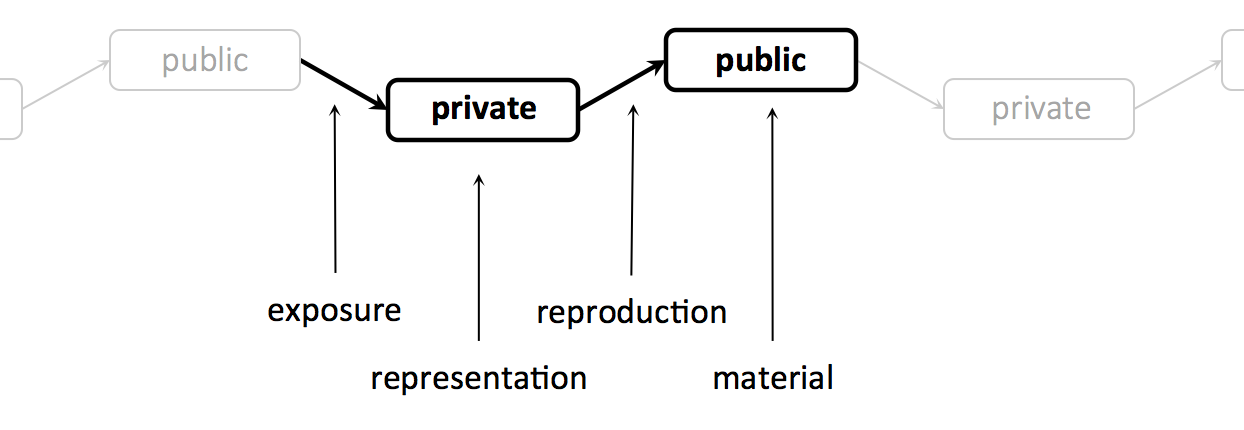
\includegraphics[width=0.95\textwidth,keepaspectratio]{figures/ch02fig02}
\caption{Loci for transmission biases; a four-stroke engine model.}
\label{fourstroke}
\end{figure}




Each of the four steps is a possible threshold for any bit 
of culture to succeed or fail in the competition for uptake in a community. If people aren't exposed to it, it will die. If it is 
difficult to remember or think of, or if in the course of mental 
representation it is radically altered, it will die, or effectively die. 
If people aren't motivated to reproduce it, no further exposure will 
happen, and when the people who have learned the practice in question die, the practice will die with them. This happens for example with language 
extinction. And if the practice is not physically realized, so that others may perceive it, the transmission process will 
stall. 



Failure on any of these four loci of transmission causes a break in the 
chain and may cause the variant to no longer exist. 



Do not get the impression that a single such chain 
represents the entire historical trajectory of a cultural item. It is 
only the tiniest strand. At any moment, there is a thicket of equivalent 
chains of iterated practice that keep a bit of language or culture alive and evolving in 
a community. 



Again, the question that a biased transmission approach 
to linguistic epidemiology asks is: What are the filters, 
pumps, and transformers that act upon the history of a cultural item? On the present proposal, we 
can posit four functionally-defined loci at which any bias can have an 
effect. Each locus is defined by the function it serves in braking, accelerating, or altering the transmission of practices in communities 
through social-cultural interaction, in an enchronic frame. 



While there may be a long, if not open list of possible biases, they all 
should be definable in terms of how they operate upon one or more of the four 
transmission loci, exhaustively defined by the causal structure 
represented in Figures \ref{iteratedpractice} and \ref{fourstroke} above: \textit{exposure} (world-to-mind transition), 
\textit{representation} (mind structure), \textit{reproduction} (mind-to-world 
transition), and \textit{material} (world structure). Within the framework of 
these basic causal loci for transmission (1-4), different biases may affect the transmission of a practice in different ways. 



As sketched above, some of these biases will have to do with facts about 
social networks, some with individual personality traits, some with 
properties of human perception, attention, memory, and action, some with 
the shape of the human body, some with the culture-specific means and 
ends that come with culturally evolved structures of activity, some with 
the organization of complex information in cognition. Let us now briefly 
consider how the previously described biases fit within 
the framework of these minimal loci for cultural transmission. Before we start, here is an important point. The goal of this exercise is not to locate each bias at just one point in the chain. As we shall see, some biases have effects at more than one point. This is one of the things the exercise shows us.


\subsection{Exposure}
\is{exposure}
Exposure --- relating to the world-to-mind transition --- is where 
biases can affect the likelihood that a person will come into contact 
with, and pay attention to, a practice.



One type of bias that effects exposure is social connectedness. All people are situated in social networks,\is{social networks} 
but they are situated in different ways. One type of difference between 
people has to do with the number of other people we come into contact with. 
\textit{Connectors} have a large number of social ties \citep{granovetter_strength_1973}. They are more likely to be exposed to an 
innovation, or to expose others to it. People with fewer social network connections will have a 
lower chance of being exposed to a given practice, or exposing others. 



Another type of bias relevant to exposure is salience.\is{salience}\is{transmission bias!salience bias}  When you come across a new kind of behaviour you may or may not pay attention to it. The things that stand out will more likely to attract your attention. The definition of \textquoteleft stand out' is 
clearly a matter of perception in the classical sense of affordances,\is{affordances} 
that is, a matter of the \textit{relationship between} a person and a thing being perceived. 
Some things are more likely to be noticed because of the nature of our 
senses in relation to the world. Other things are more 
salient to us because we are actively looking for them, often because our 
language or culture encourages or requires it.



A third bias relevant to exposure is identity.\is{identity}\is{transmission bias!identity bias}  Who is the person carrying out the practice when 
it is encountered? If it is somebody who I want to be like in some 
way, then I am more likely to pay attention to what the person is doing 
and how. If it is someone I have no interest in, I will be less likely to pay attention. In this way, social 
identity can play a role in biasing exposure, by affecting the extent to 
which someone will attend, or carefully attend, to the practice when 
encountered.


\subsection{Representation}
\is{representation}
Representation --- relating to mind structure --- is where biases can 
affect the likelihood that, or the manner in which, a practice will be 
learnt or stored by a person, or how the psychological or otherwise 
private component of a practice will be structured. 



Once we are exposed to a certain pattern of behaviour, we can 
learn it. We form a representation of it, attributing to it some meaning 
or function, and we incorporate that representation into an existing framework of knowledge. 



Some innovations\is{innovation} are more memorable than others. Some things are more easily internalized. This is explained by cognitive preferences that are either known from 
psychological science or that are on that research agenda. 



There are other differences in how things are learnt. Whether you see a thing, hear it, feel it, or some combination of these, can have 
consequences for how that thing is interpreted, learnt and understood 
\citep[Chapter 6]{enfield_anatomy_2009}. This can then affect how the new knowledge is applied. For example, it may shape how you decide that a practice 
is an appropriate means for certain ends in a particular context.



There are effects of the psychological context into which a practice is 
embedded. Practices are partly constituted by knowledge; knowledge that 
is caused by, and in turn causes, public behaviour and associated states 
of affairs. Knowledge has structure, including part-whole relations, hierarchical 
relations, and other sorts of dependency among items in a system. 



When we learn something,\is{learning} we relate it to other things we know. We do this at the 
very least because the thing stood in a certain relation to other things in the context 
in which we learnt it. As an example, if I learn a new word such as 
\textit{deplane}, I relate it to other words I already know. There might be similarities with other words: \textit{debone, derail, decode, decommission}. Or associations with other features of the language system: \textit{deplane} is a verb and 
can be used only with specific grammatical roles in English sentences.\is{English} 
Or if I learn about the possibility of downloadable ringtones I will 
naturally link this to my existing knowledge of mobile 
phones and the Internet. All of these are examples of a \textit{context bias}. Through a context bias\is{transmission bias!context bias}  a person is more readily able 
to learn and psychologically represent those things that have an 
existing \textquoteleft place' in which to fit. 



In language, items are structured into paradigms, syntagms, conceptual frames, semantic fields, and other kinds of linguistic systems.\is{systems} While these systems often display a degree of symmetry, 
consistency, and simplicity, change is always taking place. In a system, when something happens in one place 
this will have effects in another place. In lexicon and grammar, such system-internal 
dynamics\is{internal change} can give rise to a certain \textquoteleft psychological 
shakiness', as \citet{sapir_language:_1921} put it. As noted already in Chapter \ref{causaldynamics} above, this can lead to reorganization of 
a system, in people's heads, and then potentially in a whole community.



Now finally, note that \textit{content biases}\is{transmission bias!content bias}  are also relevant to the representation locus of transmission. In the broadest sense of meaning, capturing everything from the 
arbitrary meanings of words in languages to the affordance-grounded\is{affordances} 
functions of tools \citep{kockelman_residence_2006}, we benefit from what can be called 
natural meaning.\is{natural meaning} If a word or grammatical expression is compatible with 
other information, for example by having iconic properties, it is better 
learnt and remembered. Similarly for technology, if there is a good match between the intended function of a tool and the tool's natural affordances, then we are more likely to understand the practice of using that tool, it 
will be easier to learn, and indeed what needs to be stored 
in the mind is reduced because the relevant information can 
stored materially \citep{norman_cognitive_1991}. These examples of the content bias pertain to learning, storage, and 
reduction of load on cognition. 


\subsection{Reproduction}
\is{reproduction}
Reproduction --- relating to the mind-to-world transition --- is where biases can affect the likelihood that a person who is exposed to a kind of behaviour will later do it themselves. One way to think of this sense of reproduction is whatever causes a 
person to turn the private representation of a practice into an action 
whose production and effects are then perceptible by others.



What motivates us to turn knowledge into action? Daily life involves 
goal-directed behaviour that is motivated by our beliefs and desires  
\citep{davidson_essential_2006,searle_intentionality:_1983,fodor_psychosemantics_1987}. I may want to get 
something done for which I need another person's cooperation. One way to do this is with language. I select certain words and 
grammatical constructions as tools for the job. Depending on my goals, I will choose
certain words and will thereby choose against all the other words I 
could have used. 



This is the competition among words and grammatical forms invoked in 
Darwin's \citeyear[60]{darwin_descent_1871} citation of Max \citet{muller_darwinism_1870}: \textquoteleft A struggle for 
life is constantly going on amongst the words and grammatical forms in 
each language'. The competition among different cultural practices 
operates in the same way. I have a goal. I have beliefs about 
how it can be attained. I have knowledge that allows me to act. I can foresee at least some effects of my actions. All this 
points to a powerful bias at the reproduction locus of transmission, concerning a person's functional needs, and the available means to those ends. 



The content bias,\is{transmission bias!content bias}  again, fits partly under this 
rubric. As discussed above, a content bias favours a practice that is 
more beneficial in some way to the person who selects it. Recall that a direct content bias applies when the benefit is 
greater functional payoff, or reduced cost, of the practice, in 
terms of its primary functional effects. In the table tennis\is{table tennis} example (see section \ref{someknownbiases}, above), a direct content bias\is{transmission bias!direct bias}  would favour the pencil grip 
if the pencil grip were lower in cost or greater in benefit than the 
handle grip --- that is, in terms of its efficacy for getting the ball back 
over the net and, ultimately, for winning matches. An indirect content bias\is{transmission bias!indirect bias} is also relevant to the reproduction locus of transmission: the choice to use the variant at all will have to do with the effects of whom you might show yourself to identify with (or against). There is an extensive literature on this in sociolinguistics.\is{sociolinguistics} Speaking English,\is{English} I might say \textit{guy} 
in one context and \textit{bloke} in another. Maybe there is 
a slight meaning difference between these two words, thus invoking a 
direct content bias. But these differences may be minimal compared to 
the effect of identifying myself with certain sub-cultural groups or 
kinds of social relationship by virtue of this choice between different 
word forms with near-identical meanings. 



Clearer examples concern pronunciation. Whether I choose to say \textit{working} or \textit{workin'} has more to do with who I identify with 
(an indirect bias) rather than the meaning I want to convey (a direct 
bias). In the cultural realm, both a Rolex and a Tagheuer will tell the 
time for a high price but the choice to wear one or the other may depend on whether you want to 
identify with Roger Federer versus Tiger Woods (or tennis 
versus golf). 



And there is perhaps most often some combination of the two. Do I choose 
to drink this brand of beer over all the rest because it tastes better 
(a direct bias) or because by doing so I identify with some person or 
group of people (an indirect bias)? It could be both. In any case, the 
mechanisms at play will bias a person's motivation for 
selecting one practice over all the others that he thereby does not 
select. 



The indirect bias\is{transmission bias!indirect bias} is also sometimes called a model bias.\is{transmission bias!model bias} An important distinction can be made here depending on the age 
of the person concerned. How does a child select which variants of a 
practice to adopt? A conformity bias\is{transmission bias!confirmity bias} favours those practices that 
`everyone else' adopts \citep{boyd_culture_1985,gergely_sylvias_2006}. Another term for this bias is docility\is{docility} \citep{simon_mechanism_1990}. This refers to an 
adaptive propensity to do what other 
members of your group do, and in the same ways, without wondering why. An infant's model group will tend also to 
consist of the people who she is genetically most closely related to. 
The effect is that cultural practices and genes tend to (but need not) have 
parallel histories. 

As people grow up and come to be regarded full members of their group, they come across a greater number and range of cultural items. They keep learning.\is{learning} So at any time they may 
find themselves with new choices. This may be because they 
encounter other ways of doing things than the way \textquoteleft my people' do things. This happens when they come into contact with other groups, for instance in trading, 
ritual and other kinds of inter-group social interaction.\is{social interaction} Different 
people in a community will have different degrees of mobility, sometimes as a result of 
personality, sometimes as a result of gender (men often travel more 
widely than women), age or sub-culture. 



At a later age, there is a greater degree of choice and therefore 
greater competition between choices. We may or may not consciously 
deliberate about such choices. But as adults we may be more aware of the 
meanings of different options. Here is where the indirect bias\is{transmission bias!indirect bias} looks 
more like the model bias\is{transmission bias!model bias} exploited in commercial advertising. This bias applies in 
all diffusional\is{diffusion} processes by favouring practices 
that are modelled by, for example, more admired or charismatic people.


\subsection{Material}
\is{material}
Material --- relating to world structure --- is where biases can 
affect the way in which a practice will be physically perceived. 



Biases on the material locus of transmission have to do with the physical affordances\is{affordances} of cultural practices, and the ways in which these affordances affect the exposure 
and reproduction of those practices. Material-related biases can affect exposure-related biases in some 
obvious ways. The material nature of speech is such that it fades almost instantly (gesture\is{gesture} slightly less so, etc; see \citealt{enfield_anatomy_2009}).
But when language is reproduced in writing,\is{writing} this evanescence is dramatically lessened, and the 
dynamics of transmission are significantly affected. 



Outside of language, we see similar contrasts. Many activities, like adopting a certain grip for table tennis,\is{table tennis} can only be seen momentarily. They are 
only available for exposure simultaneously with the reproduction process 
that potentially constitutes the transmission event (photos, etc., 
aside). The table tennis bat itself, however, has a more persistent 
physical existence, and can stand as a public sign for the possible ways people might handle it \citep{norman_design_1988,kockelman_residence_2006}. 



Material-related biases have to do with the ways in which cultural practices are made public, and how their form of public existence might affect their availability in the 
exposure-reproduction cycle we have been exploring here.

\subsection{Networks}
\is{social networks}
If the above-mentioned elements are an engine for the tranmission of innovation, then social networks are the paths that innovations take. The career of an idea may theoretically be mapped in a large but finite network (\citealt{luce_connectivity_1950}, \citealt[Chapter 12]{miller_language_1951}, \citealt{milroy_language_1980,ross_social_1997}). 

In fashion and other kinds of social epidemic, the success of an innovation\is{innovation} will partly depend on the ways in which people's personalities\is{personality factors} differ. As \citet{gladwell_tipping_2000} accessibly lays out, different personality types contribute to the diffusion of innovation in complementary ways. Connectors have a high number of weak social connections, in a range of social spheres. Mavens are actively interested in the market, and want to share their knowledge and opinions. Salesmen are the charismatic, persuasive ones who model innovations and effectively sell them. Innovators are the risk-takers who try things before anyone else does. They are followed by early adopters, the early majority, the more conservative late majority, and finally, the laggards.

When all of these types of people come into contact, they form social networks. The approach to language in terms of networks was pioneered in sociolinguistics\is{sociolinguistics} by \citet{milroy_language_1980}, and also taken up by \citet{le_page_acts_1985}, \citet{ross_social_1997}, and others. \citet{milroy_language_1980} developed a method for studying linguistic variation\is{variation} based around the idea of social networks, \textquoteleft the informal social relationships contracted by an individual' \citep[174]{milroy_language_1980}, which \textquoteleft can be used to account for variability in \textit{individual }linguistic behaviour in communities' \citep[21]{milroy_language_1980}. The social network model \textquoteleft treats speakers as nodes in a social network, such that each speaker is connected with other speakers by social (and therefore communication) links' \citep[213]{ross_social_1997}. The idea is to map the network of contacts that each individual has. Milroy suggested that networks could be placed on a scale of density, from low to high. In a low density network, \textit{a} may be in regular contact with \textit{b}, \textit{c}, and \textit{d}, but \textit{b}, \textit{c}, and \textit{d} are never in contact with each other. In a high density network, \textit{a}, \textit{b}, \textit{c}, and \textit{d} are all in contact with each other.

Usually, contacts between two people are made in the presence of other network members. So, to the high density network, we could add the ties \textit{a-b-c, a-b-d, a-c-d, b-c-d, }and \textit{a-b-c-d}.

The network concept contributes \textquoteleft to analysis of the manner in which individuals utilise the resources of linguistic variability available to them.' \citep[175]{milroy_language_1980}. In work with Li on the topic of code-switching, Milroy writes:

	\begin{quotation} (A) network analysis can... form an important component in an integrated social theory of language choice. It links the community with the interactional level in focusing on everyday behaviour of social actors. ...  The link with the economic and sociopolitical level derives from the observation that networks seem to form not arbitrarily but in response to social and economic pressures. \citep[155]{milroy_social_1995}
	\end{quotation}
	
While \textquoteleft density' refers to the intensity of contact among network members, there are distinctions in the quality of relationships between any two network members. A distinction between \textit{exchange} and \textit{interactive} networks was suggested by \citet{milardo_families_1988}, to which Milroy and Li add \textit{passive} network ties:

\begin{quotation}
Exchange networks constitute persons such as kin and close friends with whom ego not only interacts routinely, but also exchanges direct aid, advice, criticism, and support --- such ties may therefore be described as \textquoteleft strong'.  Interactive networks on the other hand consist of persons with whom ego interacts frequently and perhaps over prolonged periods of time, but on whom ego does not rely for personal favours and other material or symbolic resources --- such ties may be therefore described as \textquoteleft weak'. An example of an interactive tie would be that between a shop-owner and a customer. In addition to exchange and interactive ties, we identified a \textquoteleft passive' type of network tie, which seemed particularly important to migrant families. Passive ties entail an absence of regular contact, but are valued by ego as a source of influence and moral support. Examples are physically distant relatives or friends. \citep[138-139]{milroy_social_1995}
\end{quotation}

The key point is that sociolinguistics and network analysis give us a valuable matrix in which a four-stroke diffusion engine operates, modulated as it is by transmission biases (see especially \citealt{rogers_diffusion_2003} for a rich review of cases and analyses of the diffusion of social innovation).

\section{Causal anatomy of transmission}



A causal explanation of linguistic reality must include the role of transmission biases in the diffusion of innovations in social networks. A good diachronic\is{diachronic frame} account of language change must be explicit about the proximal causal 
anatomy of the process, operating in microgenetic,\is{microgenetic frame} enchronic,\is{enchronic frame} and ontogenetic\is{ontogenetic frame} frames. Previous work has usefully identified and 
described transmission biases, but one might ask: Why these biases? What 
other biases might we predict are possible? How many might there be? 



We can answer these questions with reference to the basic, proximal causal anatomy of social transmission. It is powered by a four-stroke engine, a causal chain in the enchronic frame, from 
exposure to representation to replication to material instantiation, 
back to exposure and round again. A transmission 
bias is any force that serves as a filter, pump, or transformer for this 
process, with effects on any of the links in the potentially open-ended chain of iterated practice. 

A next step is to see how well we can explain the known and understood biases 
within this four-stroke engine framework, and to see what predictions can be made and tested. This should connect to research 
on the puzzle of how our species evolved\is{evolution!biological} the capacity for cumulative 
culture \citep{tomasello_cultural_1999}, a capacity that is strongly pronounced in humans but weak 
if present at all in our closest relatives, the other apes\is{apes} \citep{herrmann_humans_2007}. While we can readily assume that other animals are 
engaged in goal-directed courses of action, and that they select from 
among different means for fixed ends in both the social and material 
realms, their selection of means for ends is relatively less flexible 
than that of humans. What is the link to transmission biases? We might assume that a chimpanzee, say, will be guided in its selection 
of a behavioural strategy by a strong content bias, incorporating a 
basic min-max payoff logic: keep effort to a minimum while ensuring the desired outcome. But if its repertoire of strategies is, on 
the whole, not being acquired by learning from others --- but, say, learned by ritualization during the course of life, in an ontogenetic frame --- then transmission 
biases will have no traction. 

%To what extent do other apes possess the cognitive prerequisites for social transmission of the kind described here? While the biggest differences between us and them are known to be in social cognition, they are nevertheless intensely social species with textured societies. Many of the crucial cognitive and sociometric ingredients for biased transmission may have been in place before the evolution of our species, allowing the processes to kick in as soon as culture was being transmitted at all. 



%True reconstruction of the historical process probably a hopeless quest (Leach quote - history is not ‘irrelevant’, but ‘too difficult to put on paper’.)



 

\newpage


\chapter{The Item/System Problem}
\label{itemsystemproblem}
\is{item/system problem}


When accounts of social-cultural transmission are explicit about the 
causal processes involved, they often take cultural \textit{items} --- rather than systems --- as their unit of analysis. This works well 
but it is awkward because we know that cultural items don't exist in 
isolation. We can only make sense of cultural items in the context of a 
\textit{system} of cultural meaning.\is{systems} This brings us back to the puzzle, foreshadowed in Chapter \ref{causalunits}, of causal units. 



Higher-level systems like languages and cultures show enormous coherence 
of structure, so much so that we are seduced into thinking of them as organisms with 
bodies (see classic statements of philologists \citealt{gabelentz_sprachwissenschaft_1891} and \citealt[16]{meillet_linguistique_1926}). Here is Gabelentz:

\begin{quotation}
Language is not a mere collection of words and forms, just as the organic body is not a mere collection of limbs and organs. Both are in any stage of their life (relatively) complete systems, dependent on themselves; all their parts are interdependent and each of their vital manifestations arises from this interaction. \citep[10]{gabelentz_sprachwissenschaft_1891}
\end{quotation}

Compare this to the situation in vertebrate\is{vertebrates} 
biology. Genes\is{genetics} are distinct entities yet they \textquoteleft form 
alliances' thanks to the bodies and body plans in which they are 
instantiated (\citealt{gould_ontogeny_1977}, cited in \citealt[117]{dawkins_extended_1982}). 

\begin{quotation}
Every gene in a gene pool constitutes part of the environmental background against which the other genes are naturally selected, so it's no wonder that natural selection favors genes that `cooperate' in building these highly integrated and unified machines called organisms.  Biologists are sharply divided between those for whom this logic is as clear as daylight, and those (even some very distinguished ones) who just do not understand it --- who naively trot out the obvious cooperativeness of genes and unitariness of organisms as though they somehow counted against the `selfish gene' view of evolution. ... By analogy with coadapted gene complexes, memes, selected against the background of each other, `cooperate' in mutually supportive memeplexes. \citep[xv]{DawkinsMemeForeword1999}
\end{quotation}

Vertebrates have bodies while cultural systems 
do not. Still, the item/system link needs to be accounted for in both cases. With both bodies and memeplexes,\is{memes} sets of items somehow hold together as systems. But the causal forces are different. The pieces of a cultural system are not held together at any stage by physical 
attachment to a shared material whole. So this is our puzzle. If 
languages and other cultural systems hang together, what is the 
binding force? We have seen that cultural transmission involves causal processes that 
apply only to small parts of the larger whole. What explains the 
coherence of that larger whole? This is the item/system problem.



Here is the solution. The ideas of cultural item and cultural system are reconciled by something that they have in 
common: Neither idea exists without the simpler idea of a \textit{functional relation}.\is{functional relation} A word --- \textit{kangaroo}, for example --- is easily thought of as a 
distinct cultural item. You can cite it or borrow it without having to 
also cite or borrow the language system that it comes from. But the word 
cannot be defined or understood --- nor can it exist --- except in terms of its 
functional relation to other things, things like the words it co-occurs 
with, the conversations in which it is used for referring to kangaroos, 
and so on. The same is true for technology. A spoke\is{spoke and wheel} can be designed, named, bought, and sold, 
but as a cultural item, a spoke doesn't make sense without a wheel. And 
while a wheel is a whole when thought of with reference to a spoke, it 
is a \textit{part} when thought of with reference to a vehicle, and so 
on. 



In sum: An item doesn't make sense without functional relations to other 
things, just as a system doesn't make sense without the functional 
relations that it contains. Functional relations are the interface that 
joins items and systems together. We can look to functional relations for a solution 
to the item/system problem.

\section{A transmission criterion}

\is{transmission criterion}
In the causal ontology of culture, there is a \textit{transmission 
criterion}. A social fact --- by definition --- would cease to exist if 
individual people stopped behaving as if it existed \citep{searle_making_2010}. And social facts 
endure with relative stability beyond individual people's lifetimes. Therefore, social facts must be transmitted among individuals in human 
populations in order to (i) exist and (ii) endure with relative 
stability. Transmission is a necessary part of what makes culture and 
language the way they are. 



A causal understanding of culture depends, then, on knowing how culture is transmitted within human groups and across 
generations. Much is known about how \textit{items} are transmitted 
\citep{rogers_diffusion_2003}, but macro-level cultural systems cannot be 
transmitted in the same way. 



Do we need two separate accounts of transmission, one for items, one for 
systems? I am going to argue that we can derive system transmission from 
item transmission, on the condition that we have a more accurate 
definition of \textit{items}. We can define items not as cultural things but as 
cultural things with functional relations to other cultural things. 
Cultural items are specified for --- and advertise --- their relations to the 
contexts into which they fit (where, it must be said, this fit can be 
quickly and easily re-tooled). As \citet[19]{kockelman_agent_2013} writes: \textquoteleft there 
are no isolated environments and organisms, there are only \textit{envorganisms}.'\is{envorganism} 

\section{Defining properties of systems}

\is{systems}
To understand what a cultural system is, begin with the idea of a cultural item.\is{linguistic item} This is any seemingly detachable conceived entity such 
as a piece of technology, a technique, a way of saying something, a 
value. An item can be readily defined and labeled, and can be learned 
and borrowed from one human group into another (though typically with 
a change of meaning in the new context). Object-like 
things such as tomahawks might be prototypical items, but the idea of 
item intended here also includes train tracks, AC current, and 
mother-in-law avoidance. 



By contrast, a cultural system is a coherent \textit{set} of such items, each 
item related to the others. A system has a holism that goes 
beyond the sum of the parts, in the sense that the full meaning of any 
individual cultural item is determined by how it functions in relation to other things in context. Often, we cannot observe the system directly or in one go, as for 
example in the case of a language or a telecommunications 
infrastructure, though this is sometimes made virtually possible by 
means of \textit{signs of} these systems that scale them down in such 
a way as to produce a \textquoteleft tangible expression', as \citet[208]{durkheim_elementary_1912} put it, of the more diffuse phenomenon. 



A book can contain a grammatical description of a language. A diagram 
can portray the elements of a telecommunications system in miniature. In 
these cases a representation of the system is created or inferred 
from an aggregate of encounters with context-situated items. These 
itemized emblems are different from the real systems they 
represent, and they have different collateral effects as a result of 
their form. A grammar book,\is{grammars} for example, can be held up in one hand. This helps to promotes the idea that a 
language is a finite, bounded thing; in short, an item. 



As we now turn to examine systems in more detail let me emphasize that neither items nor systems can be understood, nor indeed can 
they exist, without the \textit{relations }that are inherent in both. 
Relations are definitive for both items and systems. If something is an item, 
relations define its \textit{functions}. If it is a system, relations 
define its \textit{structure}.



A system should have at least these three properties:\is{systems} 


\begin{enumerate}
\item It can readily be construed as a thing with multiple inter-related parts.

\item Effects on one part should have effects on other parts.

\item The parts should together form a whole in the sense that they are more closely related to each other than they are to things outside the system. 

\end{enumerate}


Good examples are biological or ecological systems. In a food chain,\is{food chain, as system} 
populations of different species are inter-related. Changes in the 
frequency or behavior of one species will affect the frequency or 
behavior of others. While each species in the ecosystem will ultimately 
be connected to entities outside the focal food chain system, the 
integration \textit{within }the system is greater. 



Clearly, on all three counts, whether or not we are looking at a system 
is ultimately a matter of construal. %(see fn. 10, above).  
To say that some entities form a system is partly just a way of looking at those 
entities. 


%\textit{note:} \textquoteleft There is evidence that grammatical change is not always limited to the language acquisition process. The grammar of an adult can change.' (H\&C:49)
%'[T]he grammar of an adult is best viewed, not as an inflexible completed object, but as an adaptable, constantly growing set of generalisations.' (H\&C:49)


\section{Relations between relations}
\is{relations between relations}

Culture and language hinge on shared meaning, and so the systems we are interested in here are \textit{semiotic }systems. The core idea of a semiotic system 
is well illustrated in Darwin's account of the expression of emotion\is{emotion} in 
animals. Darwin introduces a principle of \textit{functional connection 
}between a sign and what it stands for. 



In his example, the visible features of a dog in a \textquoteleft hostile frame of 
mind' --- upright, stiff posture, head forward, tail erect and rigid, 
bristling hairs, ears forward, fixed stare --- are intelligible because they 
recognizably \textquoteleft follow from the dog's intention to attack'. Figure \ref{darwin1} is 
Darwin's illustration.


\begin{figure}[p]
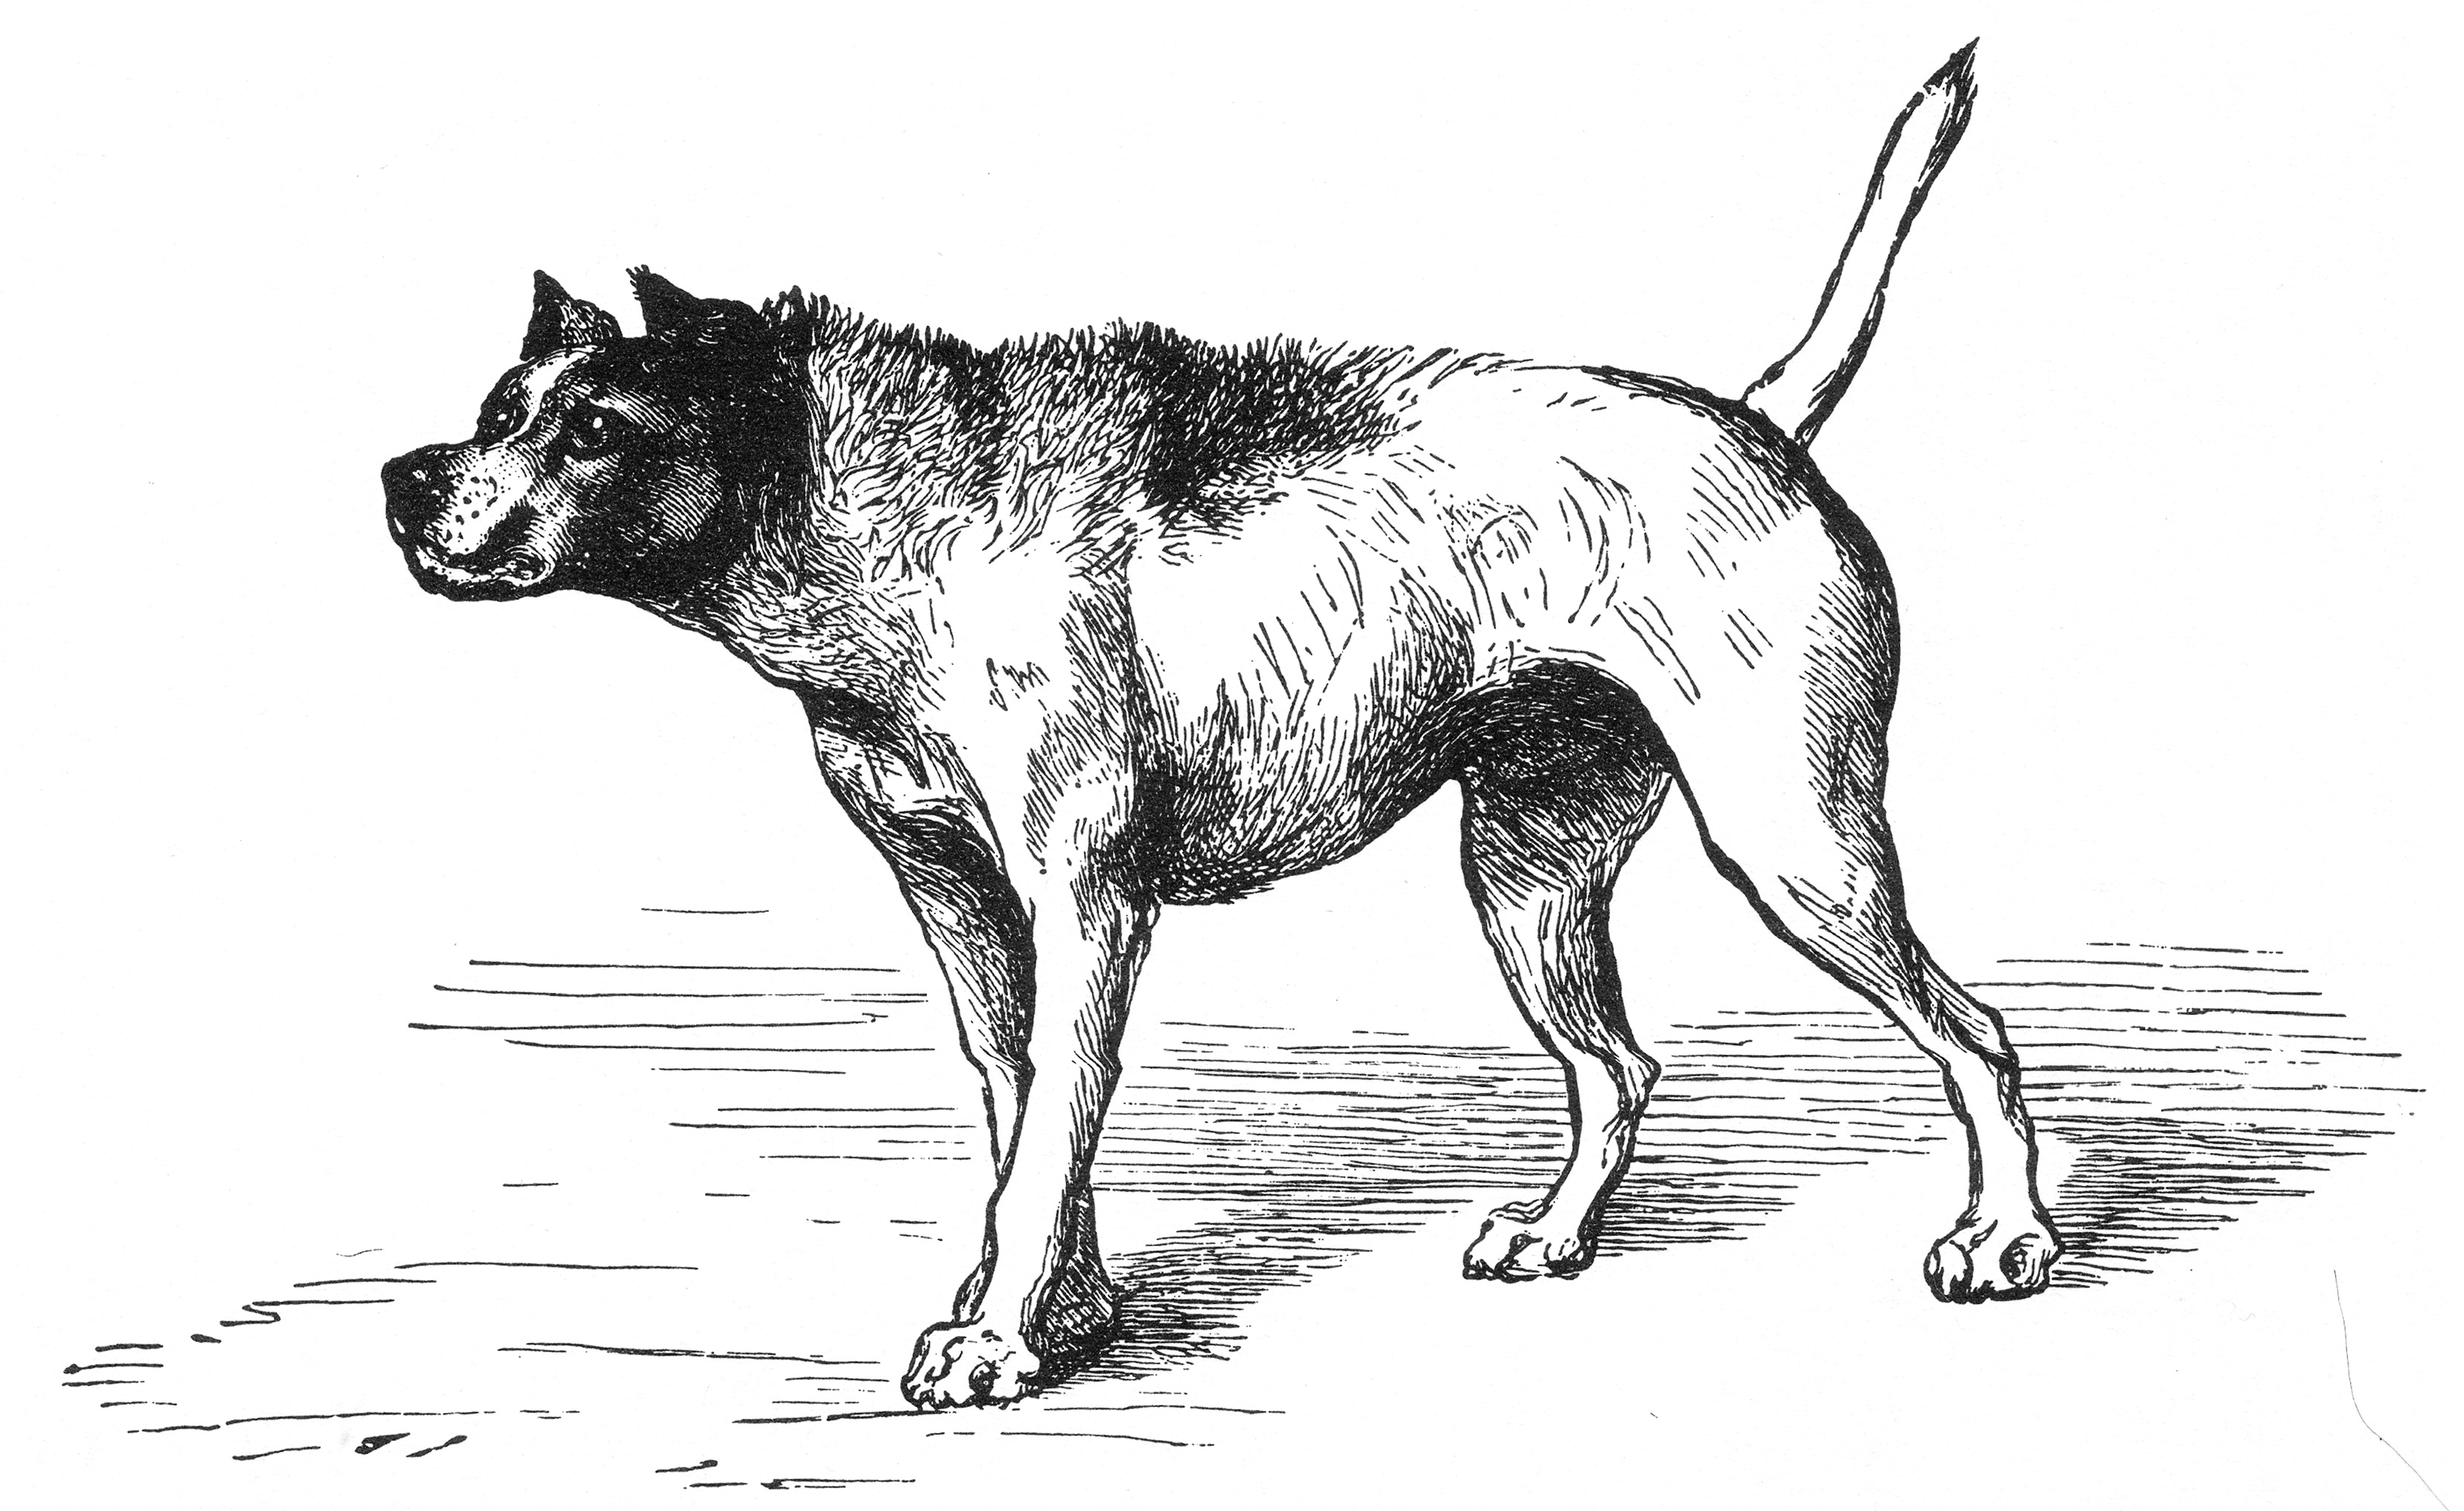
\includegraphics[width=0.70\textwidth,keepaspectratio]{figures/Fig01}
\caption{Darwin's illustration of a dog in hostile frame of mind 
(Figure 5 from \textit{The Expression of the Emotions in Man and 
Animals}).}
\label{darwin1}
\end{figure}



These behaviors are functionally connected to the aggressive attitude, 
and so others may take them to signal that attitude. This can be illustrated as in  \figref{functionalassoc}.

\begin{figure}[p]
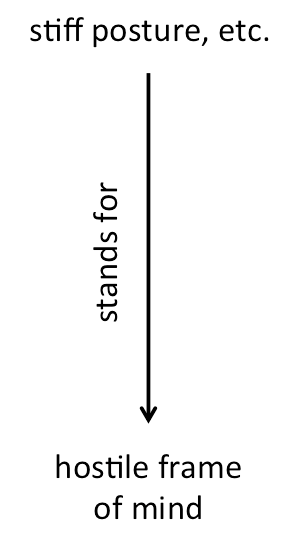
\includegraphics[width=0.22\textwidth,height=\textheight,keepaspectratio]{figures/Fig02}
\caption{A \textquoteleft functional', indexical association between observable 
behaviour and frame of mind (after Darwin).}
\label{functionalassoc}
\end{figure}


This is only a first step toward establishing a semiotic system. Figure 
\ref{functionalassoc} shows a relatively simple semiotic relation. There is a potential positive association\is{functional association} between an 
observable behavior and a frame of mind. Whoever makes this association might produce a 
number of relevant interpretants, for example running away, grabbing a big 
stick, or adopting an attacking posture. 



Darwin then argues for a second signalling principle, which he calls \textit{antithesis}.\is{antithesis} The dog can exploit the already established semiotic 
relation shown in Figure \ref{functionalassoc} to express the \textit{opposite} 
of aggression. He does this by \textquoteleft reversing his whole bearing', that is, doing the 
`opposite'\is{opposite} of what he would do when aggressive. So, when approaching 
his master in an affectionate attitude, his visible behaviors will include body 
down, flexuous movements, head up, lowered wagging tail, smooth hair, 
ears loosely back, loose hanging lips, eyes relaxed. Figure \ref{darwin2} is 
Darwin's illustration.


\begin{figure}[h]
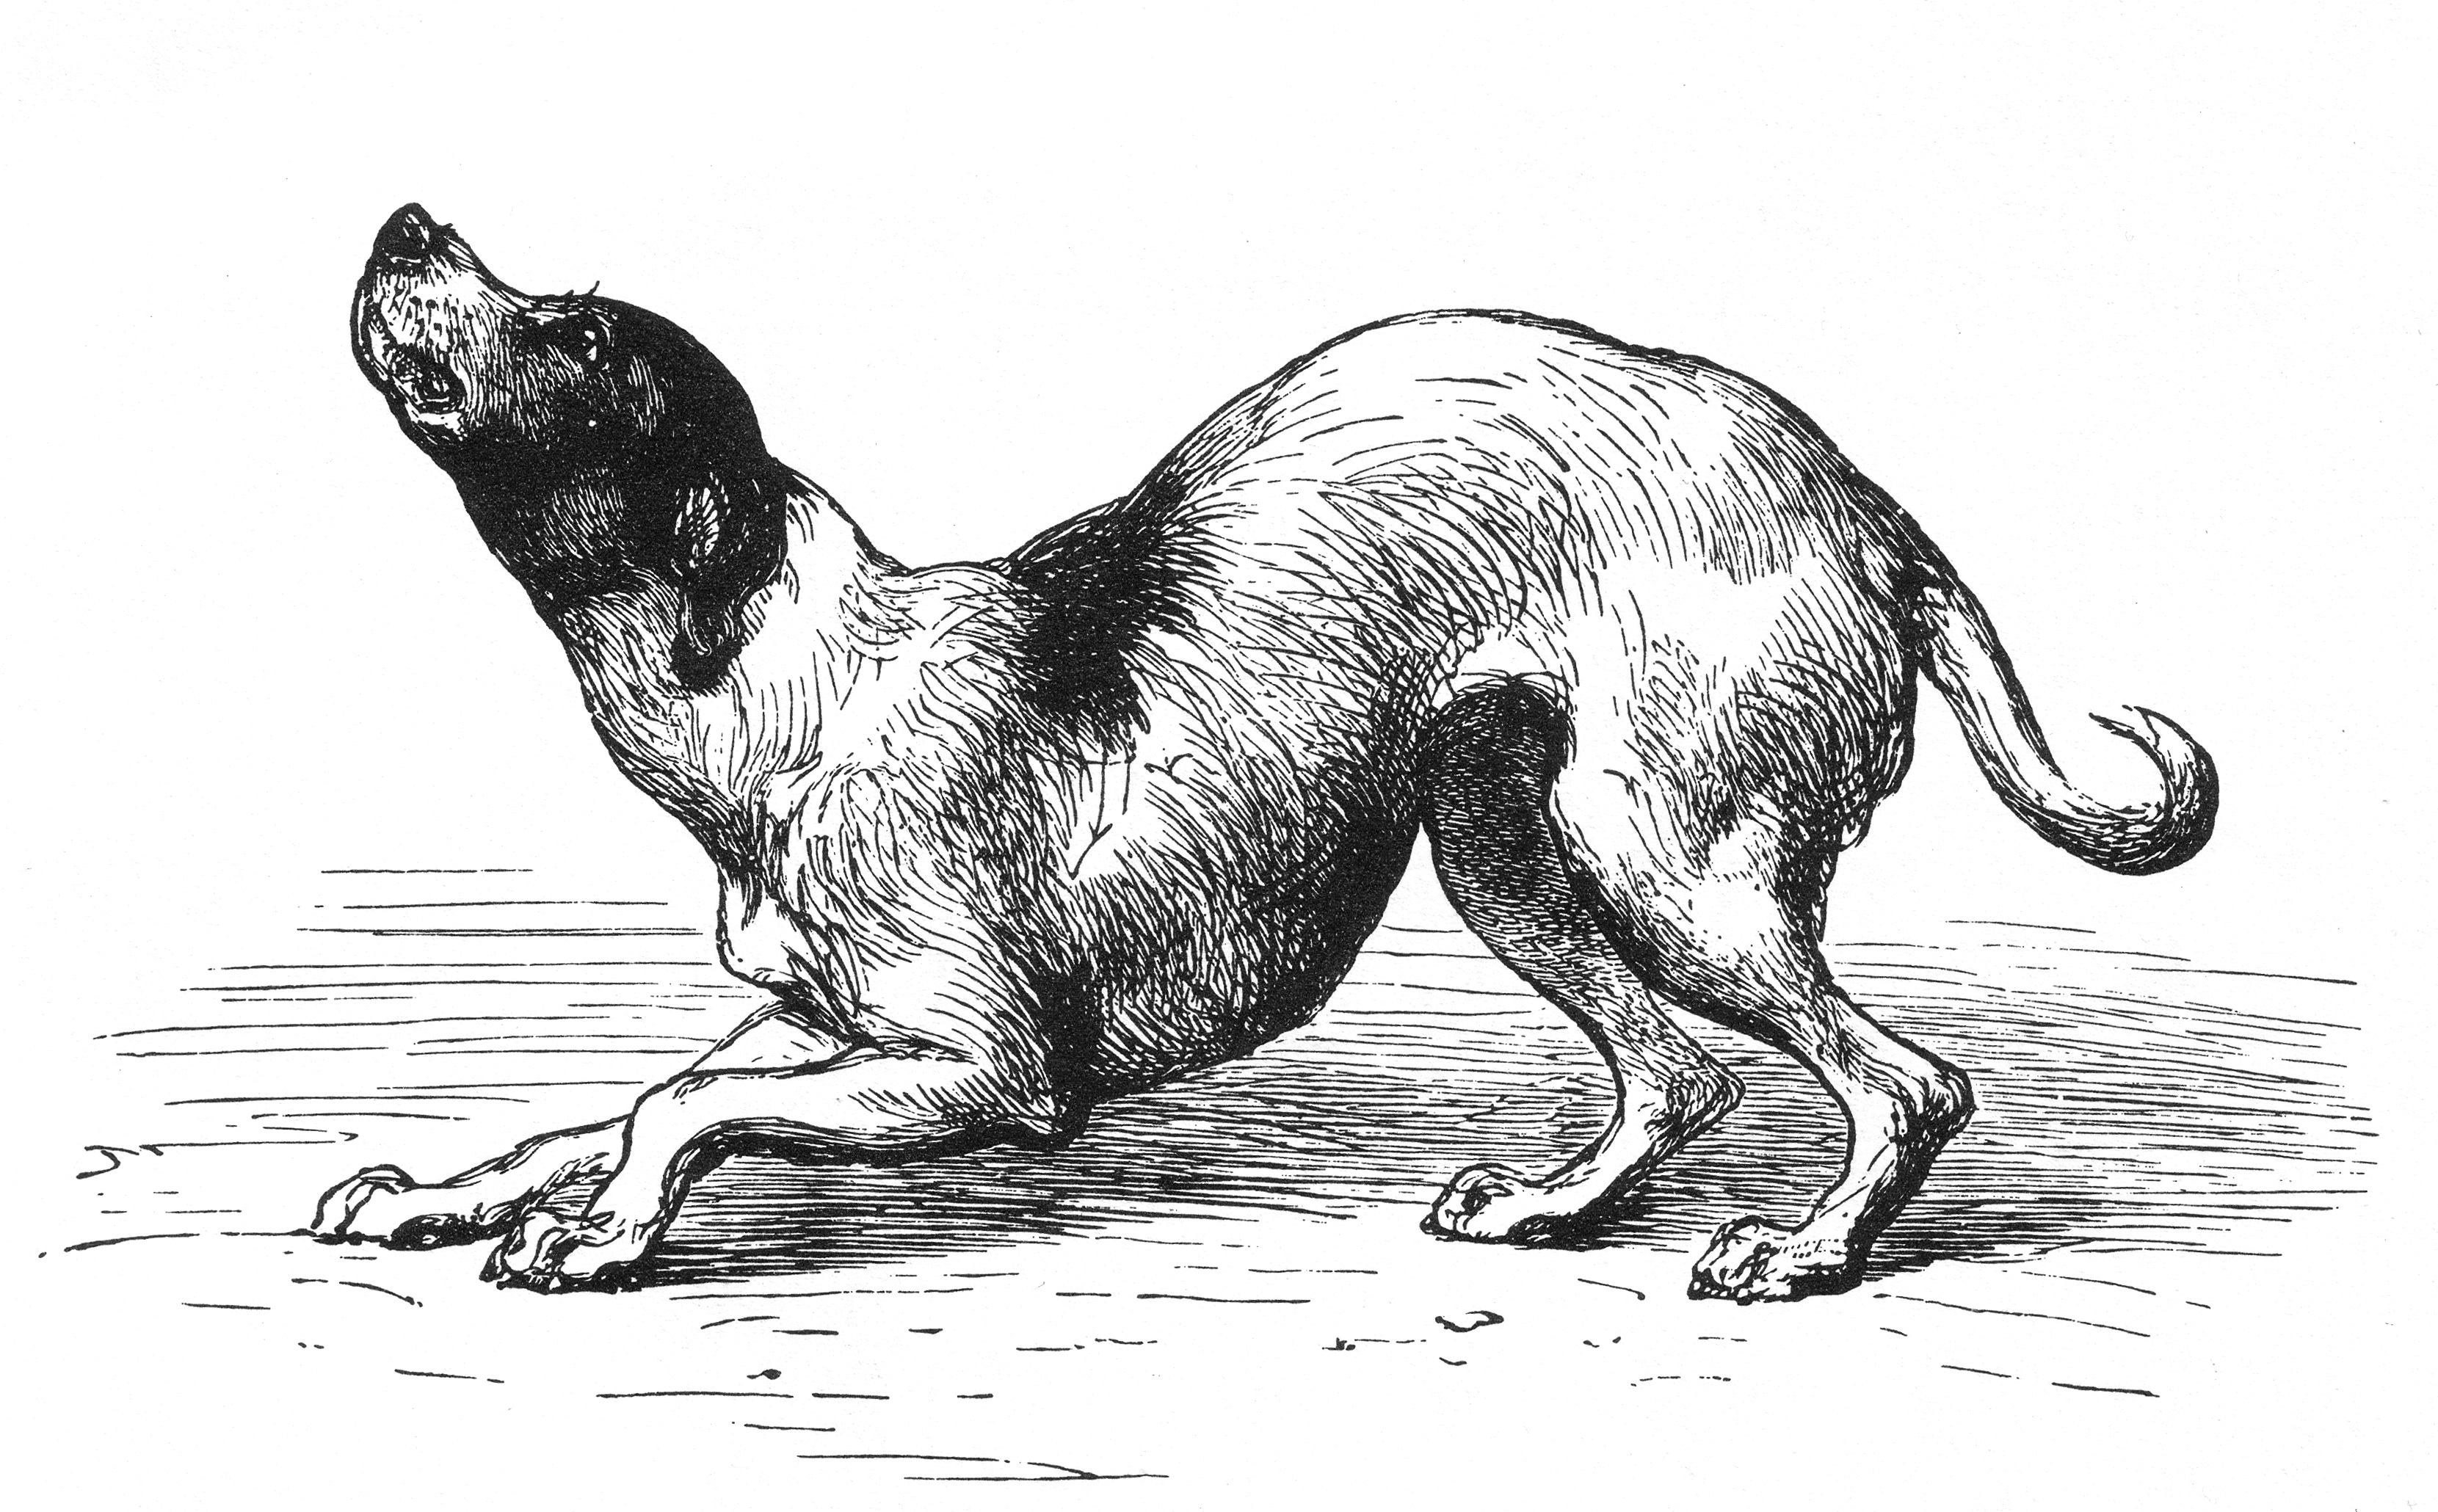
\includegraphics[width=0.70\textwidth,keepaspectratio]{figures/Fig03}
\caption{Darwin's illustration of a dog in an affectionate attitude 
(Figure 6 from \textit{The Expression of the Emotions in Man and 
Animals}).}
\label{darwin2}
\end{figure}




\begin{quotation}
None of $[$these$]$ movements, so clearly expressive of 
affection, is of the least direct service to the animal. They are 
explicable, as far as I can see, solely from being in complete 
opposition to the attitude and movements which are assumed when a dog 
intends to fight, and which consequently are expressive of anger. 
\citep[15-16]{darwin_expression_1872} 
\end{quotation}


\begin{figure}[h]
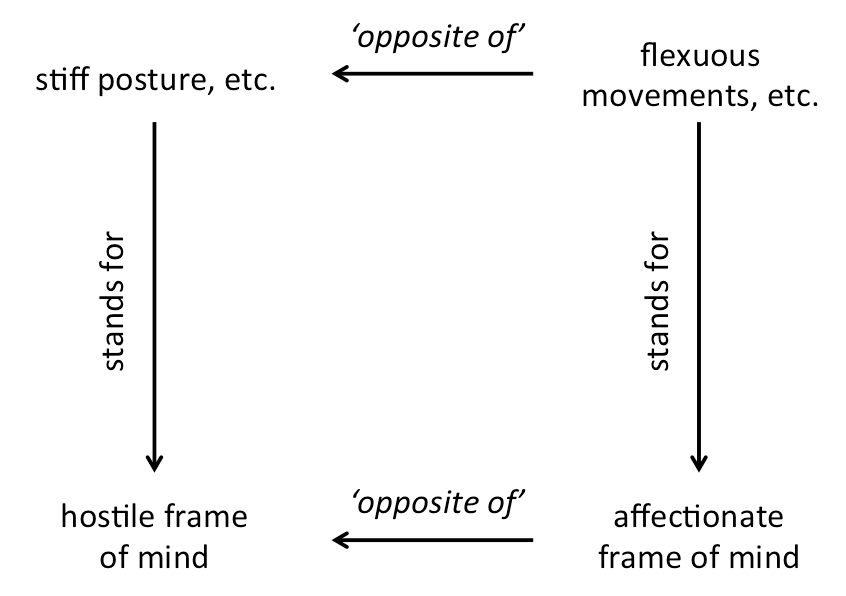
\includegraphics[width=0.55\textwidth,keepaspectratio]{figures/Fig04}
\caption{A secondary indexical association between observable behavior 
and frame of mind (at right), deriving its meaning only in connection 
with the established relation illustrated in Figure \ref{functionalassoc} (and incorporated 
at left of this Figure), assuming the interpreter's knowledge of a 
limited range of possible bodily behaviors, on the one hand, and a 
limited set of frames of mind, on the other (after Darwin).}
\label{secondaryassoc}
\end{figure}

As depicted in Figure \ref{secondaryassoc}, antithesis is a secondary relation. It is a relation between relations. As Darwin 
pointed out, this secondary relation is only possible if the interpreter has already recognized a primary functional relation. But there is something 
more that it depends on, something crucial to the idea of a semiotic 
system. It follows from the meaning of the term \textit{opposite}. 



To see that a certain behavior is `the opposite' of some 
other behavior, as opposed to simply \textit{not} that other behavior, 
you must be able to consider alternative possibilities within a 
restricted set. Flexuous movements can be recognized as the opposite of 
the aggression-signaling behavior only when one knows, or can predict, a 
limited range of postures that a dog can make. For this to work in 
the way depicted in Figure \ref{secondaryassoc}, you must also understand that there is a 
limited set of relevant frames of mind that the dog may have, with aggressive at one end and affectionate at the other. 



This type of semiotic system arises when Darwin's principle of 
antithesis sets up \textit{relations between relations} \citep[12ff]{kockelman_agent_2013}. This becomes possible when someone has access not just to what they are currently perceiving (e.g., a dog in a certain posture) but when the person also knows about other systems such as body 
posture and emotional state, with some sense of their elements 
and the logical-causal relations between them. A person should understand that if a dog is 
being affectionate it is necessarily not being aggressive, or that if 
its body is stiff it cannot also be flexuous. 



Central to the idea of a \textit{functional relation to context} that I am outlining here are the concepts of \textit{incorporation }and 
\textit{contextualization}. These are defined in semiotic terms by 
\citet[29]{kockelman_residence_2006}, as follows:



\begin{enumerate}
\item[]\textit{Incorporation.}\is{incorporation} For any two semiotic processes, A and B, A will be said to incorporate B 
(and hence be an interpretant of it) if the sign of B relates to the 
sign of A as part-to-whole, and the object of B relates to the object of 
A as means-to-ends. For example, in the case of instruments (semiotic 
processes whose sign is an artificed entity and whose object is a 
function), a wheel incorporates a spoke.



\item[]\textit{Contextualization.}\is{contextualization} For any two semiotic processes, A and B, A will be said to contextualize 
B, if A is required to interpret B, or at least assists in interpreting 
B. For example, a hammer contextualizes a nail. And a sword 
contextualizes a sheath. That is, nails make no sense without the 
existence of hammers; and sheaths make no sense without the existence of 
swords.
\end{enumerate}



The concepts of incorporation and contextualization help us to define functional relations. They hold, for example, for the relations 
between a verb and a clause, a handle and a knife, a marriage rule and a 
kinship system.\is{kinship systems} They account for relations between concepts and the larger frames that contextualize them \citep{FillmoreFrameSemantics1982}. They are the basis of combinatoric rules, and as such 
they ultimately account for grammar in the complete sense (assuming a 
semantically-based approach to grammar; cf. \citealt{langacker_foundations_1987,wierzbicka_semantics_1988,croft_explaining_2000,haspelmath_pre-established_2007}). 

%\textit{Note synchronic relations}, but realized/evidenced in microgenetic and enchronic frames; cf. also ontogenetic vs phylogenetic ritualization.

\section{More complex systems}


The basic relations-between-relations structure shown in Figure \ref{secondaryassoc} combines with incorporation and contextualization --- kinds of embedding relations --- to yield the sorts of semiotic systems that make up any natural language 
(\citealt{saussure_cours_1916}; see \citealt{dixon_basic_2010,dixon_basics_2014}, \citealt{bickel_linguistic_2014}). 



All languages have systems of form classes.\is{form classes} The thousands of 
words (and other morphemes) that you have to learn in order to 
speak a language can be categorized according to how they are
distributed relative to each other. There are open classes of 
content words like nouns and verbs (in most if not all languages) versus closed classes of function 
words like prepositions\is{prepositions} (e.g., in English)\is{English} and case-marking\is{case-marking} affixes 
(e.g., in Finnish).\is{Finnish} 



Then there are constructional systems defined by principles of combination. An example is the system for describing motion 
events\is{motion events} in Lao\is{Lao} \citep[387ff]{enfield_grammar_2007}. There are three consecutive 
slots. Each slot may be filled with a 
verb from three distinct sets. The first verb refers to the manner of 
motion (this is an open set). The second refers to the path of motion 
(from a set of 10 verbs). The third refers to the 
direction of motion in relation to the deictic centre (from a set 
of 3 verbs). See Table \ref{laodirectionalverbsystem}.


\begin{table}[htbp]
 % \centering
      \begin{tabular}{lll}
  \lsptoprule
    Slot 1 & Slot 2 & Slot 3 \\
\midrule
    Verb of manner & Verb of path & Verb of direction \\
    (open class) & (closed, n=10) & (closed, n=3) \\
    \textit{lèèn1} ‘run’ & \textit{khùn5} ‘ascend’ & \textit{paj3} ‘go’ \\
    \textit{ñaang1} ‘walk’ & \textit{long2} ‘descend’ & \textit{mùa2} ‘return’ \\
    \textit{king4} ‘roll’ & \textit{khaw5} ‘enter’ & \textit{maa2} ‘come’ \\
    \textit{lùan1} ‘slide’ & \textit{qòòk5} ‘exit’ &  \\
    \textit{tên4} ‘jump’ & \textit{khaam5} ‘cross.over’ &  \\
    \textit{lòòj2} ‘float’ & \textit{lòòt4} ‘cross.under’ &  \\
    \textit{khii1} ‘ride’ & \textit{taam3} ‘follow’ &  \\
    \textit{khaan2} ‘crawl’ & \textit{phaan1} ‘pass’ &  \\
    \textit{taj1} ‘creep’ & \textit{liap4} ‘go along edge’ &  \\
    \textit{com1} ‘sink’ & \textit{qòòm4} ‘go around’ &  \\
    \textit{doot5} ‘leap’ &       &  \\
    etc.  &       &  \\
   \lspbottomrule
    \end{tabular}%
    
\caption{Lao directional verb system}  
\label{laodirectionalverbsystem}%
\end{table}%




Using this system, a Lao speaker can say things like this:


\ea
\gll khaan2 qòòk5 paj3 \\
     crawl  exit  go \\
\glt \textquoteleft (S/he/it) crawled out/away.'
\z

\ea
\gll doot5 long2 maa2 \\
     leap descend come \\
\glt \textquoteleft (S/he/it) leapt down here.'
\z

\ea
\gll lòòj2 phaan1 mùa2 \\
     float pass return \\
\glt \textquoteleft (S/he/it) floated back past.'
\z


This linguistic sub-system illustrates a fundamental 
intersection between two axes. A \textit{syntagmatic axis}\is{syntagmatic axis} is the `left-to-right' axis along 
which separate elements combine. On a \textit{paradigmatic axis},\is{paradigmatic axis} each slot along the syntagmatic axis
may be filled by alternative members of a set, with contrast 
effects between possible values (not unlike the way a dog's stiff posture 
is opposed to a flexuous posture). 



Sub-systems in language interact with each other and show dependencies\is{dependencies in systems} 
in higher-level systems like those defined in comprehensive 
grammatical descriptions. \citet{aikhenvald_dependencies_1998} describe 
dependencies among grammatical sub-systems. They point out, for example, that 
the system of polarity\is{polarity} (positive versus negative in relation to a 
predicate or clause) puts constraints on other sub-systems in the grammars of 
many languages. For example, in Estonian,\is{Estonian} there is a system in which person and number are 
distinguished by morphological marking on the verbs, but these 
distinctions are only realised in positive polarity. The distinctions 
are lost in the negative. See Table \ref{verbtobeinestonian}.





\begin{table}[h]
\centering
\begin{tabular}{ll}
\lsptoprule
\textsc{positive} & \textsc{negative} \\
\midrule
\textit{olen} (\textsc{1sg)}, \textit{oleme} (\textsc{1pl}) 
& \\

\textit{oled} (\textsc{2sg)}, \textit{olete }(\textsc{2pl)} & 
\textit{ei ole} (1/2/3\textsc{sg/pl}) \\

\textit{on} (\textsc{3sg/pl}) & \\
\lspbottomrule
\end{tabular}
\caption{Verb \textquoteleft to be' in Estonian}
\label{verbtobeinestonian}
\end{table}


\citet{aikhenvald_dependencies_1998} present a cross-linguistic hierarchy of dependencies between sub-systems like these. This kind of inter-connectedness between 
paradigm sets and combinatoric rules, and between sub-systems in a 
language, is evidence for the broad underlying system properties of 
linguistic behavior. 



It follows from these facts about linguistic systems that we cannot 
view any piece of language as a mere item. \textquoteleft A living language is not 
just a collection of autonomous parts', say \citet[1]{donegan_rhythm_1983}. A language is \textquoteleft a harmonious and self-contained whole, massively 
resistant to change from without, which evolves according to an 
enigmatic, but unmistakably real, inner plan' \citep[1]{donegan_rhythm_1983}. 



They illustrate their point in explaining how it is that the languages 
of two sides of the Austroasiatic language family\is{Austroasiatic language family} --- Munda\is{Munda languages} and 
Mon-Khmer\is{Mon-Khmer languages} --- show a list of typological distinctions that are \textquoteleft exactly 
opposite at every level of structure' \citep[111]{donegan_south-east_2002} 
even though they are known to be descended from the same Proto language. Donegan and Stampe argue that speakers of Munda innovated a new prosodic profile, and when they did this they 
were tampering with something that \textquoteleft pervades every level of language 
structure' \citep[14]{donegan_rhythm_1983}. A simple change from iambic to trochaic\is{iambic versus trochaic} stress in words had systemic knock-on effects that changed the entire morphosyntactic profile of the language. Table \ref{mundamonkhmer}
is adapted from \citet[1-2]{donegan_rhythm_1983}.\footnote{Donegan and Stampe of course considered the possibility that language contact\is{language contact} explains the data in Table \ref{mundamonkhmer}. Their goal was to argue against a contact account, with their knock-on effect idea being offered as an alternative. Whether they are right remains an open question. Neither contact nor internal development\is{internal change} can be treated as a null hypothesis. Pronponents of both arguments are obliged to make their case.}


\begin{table}[h]
\begin{tabularx}{\textwidth}{>{\itshape}XXX}
\lsptoprule
 & \textbf{Munda} & \textbf{Mon-Khmer} \\
\midrule
Phrase accent & Falling (initial)                & Rising (final) \\[.3em]
Word order    & Variable-SOV, 
                \mbox{AN, Postpositional}        & Rigid-SVO, 
               \mbox{NA, Prepositional} \\[.3em]
Syntax        & Case, verb agreement             & Analytic \\[.3em]
Word canon    & Trochaic, dactylic               & Iambic, monosyllabic \\[.3em]
Morphology    & \mbox{Agglutinative, suffixing,} 
                 polysynthetic                   & \mbox{Fusional, prefixing} 
\mbox{or isolating} \\[.3em]
Timing        & Isosyllabic, isomoric           & Isoaccentual \\[.3em]
Syllable canon& (C)V(C)                         & \mbox{Unaccented (C)V,} 
       \mbox{accented (C)(C)V(G)(C)} \\[.3em]
Consonantism  & Stable, 
               \mbox{geminate clusters}         & \mbox{Shifting, tonogenetic,} 
       \mbox{non-geminate clusters} \\[.3em]
Tone/register & Level tone (Korku only)         & Contour tone/register \\[.3em]
Vocalism      & \mbox{Stable, monophthongal,}
       \mbox{harmonic}                & \mbox{Shifting, diphthongal,} 
\mbox{reductive} \\[.3em]
\lspbottomrule
\end{tabularx}
\caption{Properties of Munda and Mon-Khmer languages}
\label{mundamonkhmer}
\end{table} 



As the examples discussed here show, there are good reasons to believe 
that languages have higher-level system properties. Yet there is no 
single causal event in which a language as a whole system is transmitted, at least not in the same sense as the single causal event of sexual reproduction by which a full set 
of genetic\is{genetics} information is transmitted in vertebrates.\is{vertebrates} Below, I return to the 
transmission problem. But first, I want to broaden the scope and show that 
the point I have just made for language also holds for social and 
cultural systems. 



As an illustration of the system concept in another domain of culture, consider \textit{sections}\is{sections} 
and \textit{subsections}\is{subsections} in Aboriginal Australia\is{Aboriginal Australia} \citep{radcliffe-brown_social_1931}. In a 
section system, all members of a community belong in one of four 
categories. Each category has a name in the local language (e.g., in the 
Alyawarre language of Central Australia\is{Alyawarre} they are \textit{Kngwarriya}, 
\textit{Upurla}, \textit{Pitjarra} and \textit{Kimarra}). For convenience we can label them A, B, C, and D. 



As \citet[2]{mcconvell_origin_1985} describes it, in a four-term section system \textquoteleft a man 
of A marries preferentially a woman of B; their children are D. A man of 
B marries a woman of A; their children are C. C and D similarly marry 
each other, and their children are A if the mother is C and B if the 
mother is D'. After two generations of this, one ends up in the same 
section as one's father's father or mother's mother. See Figure \ref{sections}.

\begin{figure}[h]
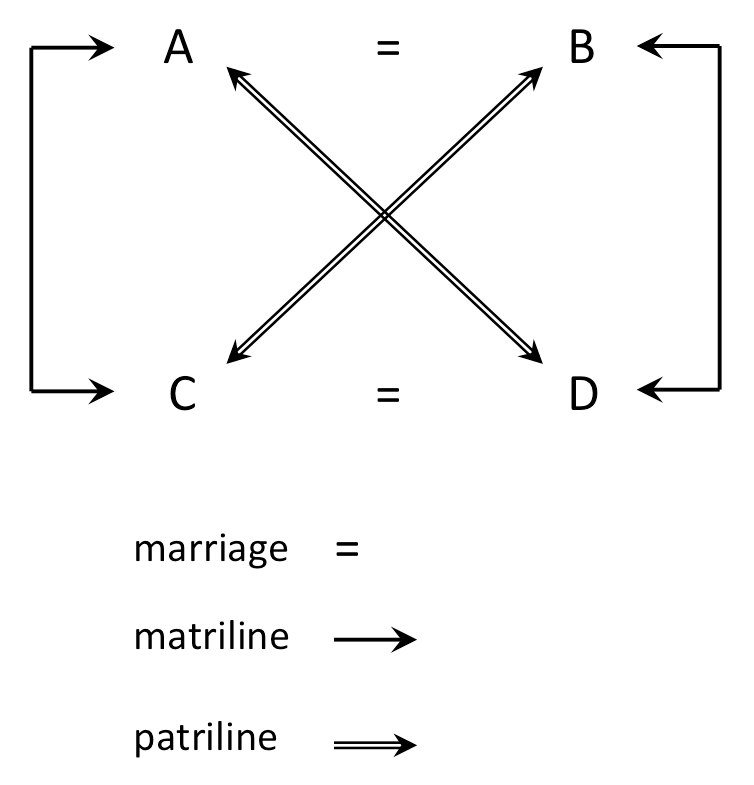
\includegraphics[width=0.5\textwidth,keepaspectratio]{figures/Fig05}
\caption{Sections (Northern Australia), from \citet[32]{mcconvell_origin_1985}, after 
\citet{radcliffe-brown_social_1931}. }
\label{sections}
\end{figure}







McConvell also describes the doubly complex subsection systems. In a subsection system, the four categories of what used to be a section system are each divided in 
two (see McConvell for diagram and discussion). There are structural 
consequences. For example, a cross-cousin is a possible wife in a 
section system, but not in a subsection system. 



These kinds of system are widespread in Aboriginal Australia. They are shared by 
groups that have completely different languages. \citet{evans_enigma_2012} compares the 
situation to that of the modern system of military ranks as officially 
standardized by the Geneva Convention:\is{Geneva Convention} groups in the same culture area have direct translations for the same offices in what is essentially the same system. In Northern Australia,\is{Northern Australia} a common cultural context has 
facilitated the widespread and stable status of particular types of 
kinship systems and vocabularies.\is{kinship systems} 



But there are many aspects of culture that seem less 
like systems and more like items. \citet{eckert_variation_2008} gives the example of a cut of 
jeans that happens to be fashionable\is{fashion} among high school kids one year, though she urges us not to be tempted by the apparent individuability of 
such cultural elements. Something like the wearing of pegged pants or a 
way of pronouncing a vowel is always situated in an \textit{indexical 
field}, as she puts it. When things like these are borrowed or adopted into new 
social settings they may be \textit{segmented} out from a historical and 
indexical constellation of signs and meanings. 



People who do this segmenting may be unaware of the larger (especially 
historical) connections. They will nevertheless give the item a 
place in a new system. \citet{parry_money_1989} make this point in connection with the historical adoption of money\is{money} around the world: \textquoteleft in 
order to understand the way in which money is viewed it is vitally 
important to understand the cultural matrix into which it is 
incorporated' \citep[1]{parry_money_1989}.



\citet{sahlins_what_1999} says that when new elements --- everything from 
money to snowmobiles\is{snowmobiles} --- are incorporated into cultural contexts, they are 
adopted for local purposes and given a \textquoteleft structural position' in \textquoteleft the 
cultural totality'. Sahlins celebrates the appropriation 
by neotraditional people of elements from other people 
(and note we can distinguish between processes of appropriation that 
alter the item so as to make it fit into the receiving system versus 
those that alter the system so as to fit the incoming item; usually it is a combination of the two). 



Sahlins is criticizing the idea that cultures like the Yupik\is{Yupik culture} 
become contaminated when people borrow modern innovations. His point is that once the items in question are borrowed, they are changed. They have new meanings in their new contexts. 



\section{Are cultural totalities illusory?}

\is{cultural totalities}
Consider the kinds of systems and relations of incorporation\is{incorporation} in language and 
culture just discussed. They show that we are never dealing with 
detached cultural items. But it does not follow from the striking 
systematicity of Australian sections\is{sections} and subsections\is{subsections} that 
these ramp up into cultural totalities. It's possible that they do. After all, ethnographers have 
succeeded in writing reference descriptions of the knowledge, practices, 
values, and technologies of defined social/cultural groups  \citep{radcliffe-brown_andaman_1922,bronislaw_malinowski_argonauts_1922,firth_we_1936,evans-pritchard_nuer:_1940,fortes_dynamics_1945}. In the same way, linguists have succeeded in describing languages as 
totalities, not in the way a layperson might discretely label an 
imagined language --- Dutch, Flemish,\is{Dutch versus Flemish} Thai, Lao,\is{Thai versus Lao} etc. --- but rather in the technical sense of listing the full vocabulary and set of 
grammatical rules that any speaker in a community should know. 



What is our evidence that such totalities exist? Both the \textquoteleft whole 
systems' and the \textquoteleft parts' of language seem clearly identifiable at first, but both ideas crumble upon close inspection \citep{le_page_acts_1985,hudson_sociolinguistics_1996}. Any linguist knows that 
\textquoteleft a language' --- in the sense of a community-wide system like French or 
Korean --- is impossible to define by pointing at 
it: \textquoteleft as a totality it is inaccessible and indefinable; each of us has 
only partial experience of it' \citep[191]{le_page_acts_1985}. 



`A language' in the sense that we normally mean it constitutes a system 
insofar as it is a set of interrelated items, such as words, each of 
which appears to be a stand-alone unit or element.\is{languages, as unit of analysis} The system\is{systems} idea is 
especially clear in the case of language for at least three reasons. First, the set of 
interrelated items in a language is a very large set. Second, we have 
strong intuitions about what is part of language and what is not. Third, this set contains numerous \textit{sub-}systems. 
But still we never encounter a language as such, only fragments of 
languages, items like words and grammatical constructions, in contexts of speech and writing. 



In their masterpiece on the nature of language, \citet[8-9]{le_page_acts_1985} challenge us to face the problem of \textquoteleft how to 
know when to speak of separate systems': 



\begin{quotation}
If we start from the concept of an underlying system this becomes an 
extremely difficult, if not insoluble, problem; if however we approach 
it from the point of view of the degree of coherence evidenced in the 
behaviour of a group of individuals, the problem is seen to be one of 
relationships and of stereotypes inherent in each individual.  
\end{quotation}




Metalinguistic stances\is{metalinguistic stances} are real. But this does not mean that the systems 
those stances point to are real in the same way. How, then, can we have a clear 
causal account of linguistic systems? The answer --- to bring us back to the 
item/system problem --- is in the causality of social behavior at the micro 
level.



%\textit{to insert}: ‘The grammar of the closed system, and its predictions of ‘grammaticality’, become confused with the empirical judgements of people whose concept of ‘grammaticality’ - if they have one at all, which is in fact comparatively rare among the world’s population at large - is subsumed within a much wider concept of ‘acceptability’, a concept which takes account of creative, innovative, analogical, inventive and tolerant capacities of the human mind ignored by the closed systems of many grammarians.’ (Le Page and Tabouret-Keller:194)




\chapter{The micro/macro solution}
\label{micromacrosolution}

Do cultural totalities exist?\is{cultural totalities} As members of a group we may feel certain that 
there is a cultural totality around us. But we never directly observe it. As 
\citet[56]{fortes_social_1949} put it:

\begin{quotation}
Structure is not immediately visible in the ``concrete 
reality''. It is discovered by comparison, induction and analysis based 
on a sample of actual social happenings in which the institution, 
organization, usage etc. with which we are concerned appears in a 
variety of contexts. \citep[56]{fortes_social_1949}
\end{quotation}

This mode of discovery is not only used by ethnographers who are studying culture.\is{culture} It is also used by children\is{children} whose task is to become competent adults (see \citealt{brown_language_2014}). 



If our experience of culture is in the micro, how do we 
extrapolate to the macro?\is{micro-macro relation} When \citeauthor{parry_money_1989} wrote about money\is{money} 
and its status, they stressed that there are local differences between cultures and the 
effects on the meaning that money comes to have. But they also acknowledged a 
certain unity across cultures: 

\begin{quotation}
[This unity is] neither in the meanings 
attributed to money nor in the moral evaluation of particular types of 
exchange, but rather in the way the totality of transactions form a 
general pattern which is part of the reproduction of social and 
ideological systems concerned with a time-scale far longer than the 
individual human life. \citep[1]{parry_money_1989} 
\end{quotation}



In terms that apply more generally to the micro/macro issue, there is ``something very general about the relationship between the 
transient individual and the enduring social order which transcends the 
individual'' \citep[2]{parry_money_1989}. It brings to mind Adam Smith's (\citeyear[book 4, ch. 2]{smith_inquiry_1776}) discussion of the relation between the 
motivations of individuals and the not-necessarily-intended 
community-level aggregate effects of their behavior \citep{schelling_micromotives_1978,hedstrom_social_1998,rogers_diffusion_2003}. \citet[29]{parry_money_1989} contrast ``short-term order'' with ``long-term reproduction'', and they suggest that the two must be linked. 



This brings us back to the transmission criterion,\is{transmission criterion} an idea that will help to bridge the micro/macro divide. If a person is to function as a member of a social group, he or she needs to individually construct, in the ontogenetic frame,\is{ontogenetic frame} the ability to produce and properly interpret the normative behavior of others.\is{normative behavior} 



Not even a cultural totality is exempt from the transmission criterion. 
Individual people have to learn the component parts of a totality during 
their lifetimes (in ontogeny),\is{ontogenetic frame} and they must be motivated to reproduce\is{reproduction} the behaviors 
(in microgeny\is{microgenetic frame} and enchrony\is{enchronic frame}) that stabilize the totality and cause it to endure beyond their own 
lives and lifetimes (in diachrony)\is{diachronic frame}. A person's motivation can be in the form of a
salient external pressure such as the threat of state violence.\is{state violence} But it usually comes from the less visible force of normative accountability\is{normative accountability} \citep{heritage_garfinkel_1984,enfield_relationship_2013}. 



In the social/cultural contexts of our daily lives, everything we do will be interpreted as meaningful. ``The big question is not whether 
actors understand each other or not'', wrote \citet[367]{garfinkel_perception_1952}. ``The fact is that they do understand each other, 
that they \textit{will} understand each other, but the catch is that 
they will understand each other regardless of how they \textit{would} 
be understood.'' This means that if you are a member of a social group, you are not 
exempt from having others take your actions to have meanings, whether or 
not these were the meanings you wanted your actions to have. 



As \citet[321]{levinson_pragmatics_1983} phrases it, also echoing Goffman and Sacks, we 
are ``not so much constrained by rules or sanctions, as caught up in a 
web of inferences'.\is{web of inferences} We will be held to account for others''
interpretations of our behavior and we know this whether we like it or 
not.\footnote{This does not mean that we are accountable for just any interpretation, but only those interpretations that are grounded in social norms. For example, if you are in the habit of going barefoot on the street, you can expect people to draw attention to this whether you like it or not (in a way that they will not if you are in the habit of wearing shoes).} This is a powerful force in getting us to conform. Accountability 
to norms ``constitutes the foundation of socially organized conduct as a 
self-producing environment of `perceivedly normal' activities''
\citep[119]{heritage_garfinkel_1984}. The thing that tells us what counts as normal is of 
course the culture.\is{culture} 



\begin{quotation}
With respect to the production of normatively appropriate conduct,\is{normative behavior} all 
that is required is that the actors have, and attribute to one another, 
a reflexive awareness of the normative accountability\is{normative accountability} of their actions. 
For actors who, under these conditions, calculate the consequences of 
their actions in reflexively transforming the circumstances and 
relationships in which they find themselves, will routinely find that 
their interests are well served by normatively appropriate conduct. With 
respect to the anarchy of interests, the choice is not between 
normatively organized co-operative conduct and the disorganized pursuit 
of interests. Rather, normative accountability is the ``grid'' by 
reference to which \textit{whatever} is done will become visible and 
assessable. \citep[117]{heritage_garfinkel_1984}
\end{quotation}



One might ask what is ``normatively appropriate conduct''. The answer must 
include any of the kinds of behaviors discussed in the above section on 
cultural systems: for example, behaving in accordance with the rules of 
a section\is{sections} system by marrying someone of the right category (or being 
able to give reasons why you have done otherwise). They would 
not be cultural behaviors if they were not regimented in a community by 
accountability to norms (and probably also laws). 



So the path that is both the least resistant and the most empowering for 
a person is to learn the system that generates a shared set of 
normative interpretations of people's behavior, and then go with the 
flow. This is how the totality cannot exist without the individuals, 
while -- paradoxically -- appearing to do just that. We create and maintain the very systems that constrain us.



The close relationship between short-term order and long-term 
reproduction is an asymmetrical one. Short-term order is where the 
causal locus of transmission is found. It is where acceleration, 
deceleration, and transformation in cultural transmission occurs 
\citep{schelling_micromotives_1978,sperber_anthropology_1985,sperber_explaining_1996,rogers_diffusion_2003}. 



From all of this it is clear that cultural systems exist and they both 
constrain us and guide us. The question is: How are systems transmitted? The regulation of individual behavior in the cultural 
totality is not achieved by mere emergence.\is{emergence} It is not like the self-oriented behavior of a bird 
in the seemingly concerted movement of a flock. Individuals' behavior 
is regulated by norms, in an effectively telic way. A good deal of 
cultural regimentation is done through explicit instruction, often with 
reference to norms, and sometimes with reference to punishable laws. 



To see how whole cultural systems are transmitted, we have to draw on item-based processes of transmission. As we 
saw in the last chapter, the only good causal account we have for social 
transmission through populations and across generations is one that 
works in terms of items, not whole systems.



\section{The combinatoric nature of cultural items in general}


Recall that the context bias\is{transmission bias!context bias} is grounded in the fact that one cannot 
behold any so-called item without beholding it \textit{in relation to}
something else, including not only things of similar kinds, but also the social norms and intentions associated with items and 
the contexts in which they appear. So, I cannot know what a hammer is if I do not see it in relation to the human body, 
timber and nails, people's intentions to build things, conventional 
techniques for construction, and so on. 



These relations -- which themselves are interrelated -- form an indispensible 
part of what I am referring to by the term \textit{item}.\is{linguistic item} When a cultural item 
diffuses, what is diffusing is something less like an object 
and more like a combinatoric relation. So, a hammer incorporates a 
handle or grip. The handle or grip has a combinatoric relation to the 
human hand insofar as the handle and the hand are practically and 
normatively designed to go together. The handle is designed that way 
because of how the human hand is. The handle only makes sense in terms 
of a person's hand. 



This going together of the handle and the human hand is like a grammatical 
rule. In a similar way, the handle of the hammer and the \textit{head} of the 
hammer go together both 
practically and normatively. The head of the hammer, in turn, goes with a nail. The nail, in turn, goes with timber, and so forth. So we see how the cultural items that diffuse in communities necessarily 
incorporate -- and advertize -- their rules of fit with other items. 



The sprawling yet structured systems\is{systems} that we call languages\is{languages, as unit of analysis} have the same kinds of properties of incorporation\is{incorporation} and contextualization\is{contextualization} that I 
have just described for concrete objects. So, if speakers of a 
language have borrowed\is{borrowing} a word from another language, this does not mean they have 
merely adopted a pairing of sound and concept. They must also have adopted a way of relating the word to their existing language system 
(whether or not this relation resembles the one used in the source 
system). 



The word will not be usable if it does not have combinatoric properties that specify how it fits with other words. 
The norms for combining the word in usage may be borrowed along with the 
word itself, or they may be provided by existing structures in the borrowing 
language, or they may even be innovated in the process of incorporation.\is{incorporation} 



The combinatoric relations surrounding a cultural item 
do not have to diffuse along with that item. But a cultural 
element must have \textit{some} 
combinatoric relation to other cultural items in the same domain if it is to function and circulate. That relation can just as well be invented by the people who adopt the item, in line with the contraints of their own culture and world view. This 
is the point that authors like Sahlins and Eckert, mentioned above, 
have stressed for culture.



So, structuralist linguists like \citet[1]{donegan_rhythm_1983} are right when they 
say that a language ``is not just a collection of autonomous parts''. But
this does not mean that a language is ``a self-contained 
whole''. The same applies when cultural anthropologists 
refer to the ``cultural totality''.\is{cultural totalities} 



We never encounter whole systems except one fragment at a time, in microgeny\is{microgenetic frame} and enchrony.\is{enchronic frame} Our 
``partial experience'' \citep[191]{le_page_acts_1985} is not 
experience of the whole system. But nor is it experience of stand-alone 
items. When we experience culture, we experience meaningful items in 
relations of functional incorporation\is{incorporation} and contextualization\is{contextualization} with other 
such items. 


Each such relation is, effectively, a combinatoric principle, like a 
norm for forming a grammatical sentence or for using a hammer and nail 
in the appropriate way. These relations are at the center of the 
framework being proposed here. These relations are what is transmitted. 
They have an inherent connection to a cultural system or field, 
but this system or field has no pre-given size or outer borderline.



\citet{bloch_well-disposed_2000} says that old critiques of diffusionism\is{diffusionism} in anthropology 
also work as critiques of today's item-based accounts. I would say that 
the problems are handled by the simple conceptual shift 
being proposed here. The relevant unit of cultural transmission (meme\is{memes} or 
whatever) is not \textit{a piece}. The relevant unit is \textit{a piece and its 
functional relation to a context}. This might seem obvious. But when we 
make it explicit, the fear of a disembodied view of cultural units goes 
away. The required conceptual move is not to take 
items and put them in a context. Their relation to a context is what \textit{defines} them. 



\section{Solving the item/system problem in language}


Identifying the \textit{relation to context} as the common unit of 
analysis of both items and systems is necessary but not yet sufficient. We 
need an account of how this scales up into large structured sets of such 
relations. Let us consider the question in connection to language. Every linguistic convention in a community is a 
product of general mechanisms of social diffusion.\is{diffusion} Each convention has its own history. Every word, 
every morpheme, every construction has followed its own historical path to 
community-level acceptance. As \citet[444]{bloomfield_language_1933} said, ``individual forms may have had very 
different adventures''. 



This does not mean languages are mere bundles 
of items. They are large, structured, systematic wholes. Psychologically, languages exist in people's minds and bodies.
They take the form of idiolects.\is{idiolects} Intersubjectively, 
languages exist at a \textit{community} level to the extent that people's 
idiolects are effectively alike in structure and content, as 
demonstrated by the evidently tolerable degree of success 
of communication \citep{enfield_utility_2015}. 
\enlargethispage{1em}
We can now 
specify some forces that bring items together and structure them into 
systems.



\section{Centripetal and systematizing forces}

\is{centripetal forces on items}
When we say that two people speak the same language, we mean that two individuals' knowledge of a language system -- synchronically,\is{synchronic frame} as can be seen in their enchronic\is{enchronic frame} and microgenetic\is{microgenetic frame} behavior -- is effectively (though never exactly) shared. This sharedness exists because a large number of the same linguistic variants have been channelled, in a huge set, along the same historical pathways. This gives the impression that a language is passed down as a whole, transcending lifetime after lifetime of the individuals who learn and embody the system. 



This is the point made by \citet{thomason_language_1988}: Normal social 
conditions enable children, as first language learners,\is{first language acquisition} to construct 
idiolects that effectively match the idiolects of the people they learn 
from -- i.e., those with whom children share a household and an immediate social 
environment, and who are, incidentally, most likely to share their 
genes. Normal transmission\is{normal transmission} is what allows historical linguists\is{historical linguistics} to 
abstract from the fact that each linguistic variant has its own career, 
and in turn to treat the whole language as having one 
spatial-historical trajectory.



In many cases this is a reasonable and successful methodological 
presumption \citep{haspelmath_how_2004}. But in 
situations other than those of normal transmission\is{normal transmission} \citep{le_page_acts_1985,thomason_language_1988}, linguistic items do 
not always travel together, but may follow separate paths, making 
visible what is always true but usually obscured by items' common 
destiny in practice, namely: Each item has its own history. 



Genealogical continuity in language change\is{language change} is typically taken to be the 
norm. Whenever we see that linguistic systems\is{systems} are permeable, for instance in certain language contact situations where the 
components of languages are prised apart, special explanations are 
demanded. 

\section{On normal transmission}

To say that a child inherits a language from her parents is a misleading representation of what happens in language acquisition.\is{first language acquisition}\is{ontogenetic frame} The idiolect of the child is not acquired like DNA in a bundle.\is{genetics} Patterns of constituency and grammatical relations do not unfold in children like the shapes of their bodily organs. Through practice, children have to learn, construct, and maintain skills and ideas for ways of saying things. 

\begin{quotation}
The ``rules'' of a child's ``native language'' ... are in any case likely to be tentative hypotheses, easily modified by fresh semantic needs, fresh contacts, fresh analogies. ``Syntax'' in the grammarian's sense is what emerges from this process, not what it starts from. \citep[190]{le_page_acts_1985} 
\end{quotation}

\begin{quotation}
Logic and universal grammar, then, are targets towards which, rather than the starting point from which, human linguistic activity proceeds. The origins of that activity are like those of a game which gradually develops among players, each of whom can experiment with changes of the rules, all of whom are umpires judging whether new rules are acceptable. \citep[197]{le_page_acts_1985} 
\end{quotation}

This transmission takes place through air, over days, weeks, months, years, with interference and noise. Every bit of the idiolect's structure has to be passed over and constructed from scratch by the learner. This task is made possible by the sheer deluge of linguistic data -- a \textit{Niagara of words}, as \citet[12]{hayakawa_language_1978} called it -- which people are exposed to, and produce in turn. Child language acquisition is a process of building \citep{tomasello_constructing_2003}, resulting in something like a grammatical totality in the child's competence.\is{competence} But whatever totality a person has built, it is instantiated somehow in the head and so (a) will never go public as a whole and (b) will be destroyed when the person dies. The system is neither observed nor passed on as a whole unit, only ever fragment-by-fragment.

\citet{dunbar_grooming_1996} has hypothesized that prelinguistic human ancestors created language\is{evolution!of language} as a way to lessen time pressure due to the need to manage an expanding number of social associates. Sustaining a social network\is{social networks} by means of linguistic contact is time-consuming. Where personal exchange or strong network ties are involved, we are necessarily oriented towards a limited group. The size of networks is constrained by the time it takes to maintain these relationships. However, the number of non-personal exposure ties -- passive seeing and hearing, especially due to media and high population density -- is potentially massive. The invention of writing has drastically changed the proportion of personal and non-personal sources of exposure to innovation.

\citet{thomason_language_1988} invoke an idea of \textit{normal transmission} (see above). They define normal transmission\is{normal transmission} ``by exclusion'' \citep[10]{thomason_language_1988}, in terms of how ``perfectly'' all sub-systems of a language are reproduced in children's idiolects. In normal transmission, linguistic input from outgroup people has negligible impact on a child's construction of an idiolect highly convergent with the idiolects of the parents' generation. 
Normal transmission, in Thomason and Kaufman's sense, is a social fact \citep[12]{thomason_language_1988}, though it is defined by formal facts about child language acquisition in a community:

\begin{quotation}
[A] claim of genetic relationship [between a ``parent'' and a ``daughter'' language] entails systematic correspondences in all parts of the language because that is what results from normal transmission: what is transmitted is an entire language -- that is, a complex set of interrelated lexical, phonological, morphosyntactic, and semantic structures. \citep[11]{thomason_language_1988}
\end{quotation}
	
Here is how I understand Thomason and Kaufman's point. To say that a ``genetic'' relationship holds between parent and daughter languages is to use a metaphor, and to use this metaphor is harmless as long as the older generation's idiolects are reproduced so closely in the idiolects of the younger generation that it is \textit{as if} the new idiolects were replicas of the old. This is effectively what happens in the case of normal transmission. There is a relentless and focussed linguistic sign deluge from people of the learner's own group.



But another question remains. How can we explain the relative impermeability of linguistic systems in circumstances of normal transmission? Stability in conventional systems\is{systems} is no less in need of 
explanation than variation or change \citep{bourdieu_outline_1977,sperber_explaining_1996,sperber_cognitive_2004}. What are the forces that cause linguistic variants to follow en masse a single path of diffusion 
and circulation, and to hold together as structured systems? Let us briefly 
consider three such forces.



\subsection{Sociometric closure}
\label{sociometricclosure}

\is{sociometric closure}

A first centripetal force is sociometric closure. This arises from a trade-off between strength and number of relationship ties in a 
social network.\is{social networks} If a person is going to maintain a social relationship, she 
has to commit a certain amount of time to this. Time is a 
finite resource. This puts a structural constraint on the possible 
number of relationships one can maintain \citep{hill_social_2003}. 
The result is a relatively closed circulation of currency within a 
social economy of linguistic items. It causes people's inventories of 
items (i.e., their vocabularies, etc.) to overlap significantly, or to 
be effectively identical, within social networks.



This helps to account for how people who interact often
can have a common set of variants. It does not account for the 
system-like nature of the relations among those items. We 
turn now to two forces of systematization inherent 
to grammar, in the paradigmatic\is{paradigmatic axis} and syntagmatic axes.\is{syntagmatic axis}



\subsection{Trade-off effects}
\label{tradeoff}

\is{trade-off effects}
One systematizing force comes from functional trade-off effects that 
arise when a goal-oriented person has alternative means to similar ends. When different items come to be used 
in a single functional domain, those items can become formally and 
structurally affected by their relative status in the set. This happens 
because the items compete for a single resource, namely, our selection of 
them as means for our communicative ends. 



When \citet{zipf_human_1949} undertook ``a study of human speech as a set of 
tools'', he compared the words of a language with the tools in an 
artisan's workshop. Different items have different functions, and different relative functional loads. In a vocabulary, \citet[21]{zipf_human_1949} 
argued, there is an internal economy of words, with trade-offs 
that result in system effects like the observed correlation between 
the length of a word (relative to other words) and the frequency of use 
of the word (relative to that of other words).\is{length-frequency rule} 



Zipf reasoned that ``the more frequent tools will tend to be the lighter, 
smaller, older, more versatile tools, and also the tools that are more 
thoroughly integrated with the action of other tools'' \citep[73]{zipf_human_1949}. He 
showed that the more we regard a set of available means as alternatives 
to each other in a functional domain, the more they become defined in 
terms of each other, acquiring new characteristics as a result of their 
role in the economy they operate in. In other words: The more we 
treat a set of items as a system, the more it becomes a system.\is{systems}



\subsection{Item-utterance fit, aka content-frame fit}
\label{itemutterance}
\is{item-utterance fit}\is{content-frame fit}

A final key source of grammatical structure is grammatical 
structure itself. The \textit{utterance }is a core structural locus in 
language. An utterance is a local context for the interpretation of a 
linguistic item. It is an essential ratchet between item 
and system. As Kirby writes, although ``semantic information'' is what 
linguistic utterances most obviously convey, ``there is another kind of 
information that can be conveyed by any linguistic production, and that 
is information about the linguistic system itself''.

\begin{quotation}
When I produce the sentence ``these berries are good'' I may 
be propagating cultural information about the edibility of items in the 
environment via the content of the sentence. At the same time I may also 
be propagating information about the construction of sentences in my 
language. \citep[123]{kirby_transitions:_2013} 
\end{quotation}
%(Kirby 2013, 123). 

In this way, an utterance is a frame and a vehicle for replicating linguistic variants \citep{croft_explaining_2000}. 



Item-utterance fit is the structural fit between diffusible types of 
linguistic items and the token utterances in which they appear. It is an 
instance of the more general \textit{content-frame} schema \citep{levelt_speaking:_1989} also 
observed in phonology (MacNeilage \citeyear{macneilage_frame/content_1998}; see \citealt[54--55]{enfield_relationship_2013}), and a 
case of the ``functional relation to context'' defined above as a common property of items and systems. Now we see that it is not just a 
common property. It is the very property that connects items with systems. An utterance is an incorporating\is{incorporation} and contextualizing\is{contextualization} 
frame for the diffusion of replicable linguistic items,\is{linguistic items} \textit{and} it is a frame for the diffusion of the combinatoric rules from which the 
higher-level system\is{systems} is built. 



\section{A solution to the item/system problem?}


The above considerations suggest that the item/system problem\is{item/system problem} can be 
solved if the following three forces apply in the 
biased transmission of cultural items: 

\begin{enumerate}

\item {\textit{Congregation:} Items are brought together and ``bundled'' by the population-level effects of inward-directed sociometric biases.}

\item {\textit{Specialization:} Items then effectively compete for selection in the same functional contexts, and come to be specialized as alternative means for related functional ends.}
 \item {\textit{Combination:} Items in a set come to combine with each other in functional ways, via context biases and the relation of item-utterance fit.} 

\end{enumerate}

We can expect there to be analogous relations to 
item-utterance fit  (=content-frame fit) in the domain of culture. Think, for instance, of 
systems of social relations in kinship,\is{kinship systems} or systems of material culture 
and technology in households and villages. 



Zipf's (\citeyear{zipf_human_1949}) analogy is useful here. For his ``economy of tools-for-jobs 
and jobs-for-tools'' to get off the ground, one first needs a \textit{workshop}, somewhere the set of tools is assembled in one place, 
and made accessible to a person with goals. In language and 
culture, this is achieved by sociometric closure\is{sociometric closure} (\sectref{sociometricclosure}, above): the more you talk with certain people, the more ways of talking you will share with these people. 
Then, one works with the set of tools, using them as alternative specialized means to similar or related ends (\sectref{tradeoff}, above). Finally, these tools will, whether 
by design or by nature, enter into the relations of incorporation\is{incorporation} and 
contextualization\is{contextualization} that define their both their functional potential and their system status (\sectref{itemutterance}, 
above). 



Now this should look familiar to the linguist. Once we get an \textit{inventory} or lexicon of items that have specalized functions within a given domain, they will naturally enter into the 
\textit{paradigmatic}\is{paradigmatic axis} and \textit{syntagmatic}\is{syntagmatic axis} relations that 
define semiotic systems\is{systems} in the classical sense.









\newpage
\chapter{Conclusion}



Ever since Darwin's\is{Darwin} earliest remarks on the uncanny similarity between 
language change\is{language change} and natural history in biology\is{evolution!biological}, there has been a 
persistent conceptual unclarity in evolutionary approaches to cultural 
change. This unclarity concerns the units of analysis. 



In some cases the unit is said to be the language system as a whole.\is{languages, as unit of analysis} A 
language, then, is ``like a species'' (\citealt[60]{darwin_descent_1871}; cf. \citealt[192--194]{mufwene_ecology_2001}). If so, then we are talking about a population 
of idiolects\is{idiolects} that is coterminous with a population of bodies (allowing, 
of course, that in the typical situation -- multilingualism\is{multilingualism} -- one body houses 
more than one linguistic system). 



On another view, the unit of analysis is any unit that forms \textit{part} of a language, such as a word or a piece of grammar.\is{linguistic items} ``A struggle 
for life is constantly going on amongst the words and grammatical forms 
in each language'' (\citealt{muller_darwinism_1870}, cited in \citealt[60]{darwin_descent_1871}). By
contrast with the idea of populations of idiolects, this suggests that 
there are populations \textit{of items }(akin to Zipf's economy of 
word-tools), where these items are produced, and perceived, in the 
context of spoken utterances. 



While some of us instinctively think first in terms of items,\is{linguistic items} and others 
of us first in terms of systems,\is{systems} we do not have the luxury of ignoring either. 
Neither an item nor a system can exist without the other. The challenge 
is to characterize the relation between the two. This relation is the 
one thing that defines them both. 



The issue is not just the relative status of items and systems but the 
causal relations between them. If the distinction 
between item and system is a matter of framing, it is no less 
consequential for that. We not only have to define the differences 
between item phenomena and system phenomena, we must know which ones we 
are talking about and when. And we must show whether, and if so how, we 
can translate statements about one into statements about the other. 

\section{Natural causes of language}


``We might gain considerable insight into the mainsprings of human 
behavior'', wrote \citet[v]{zipf_human_1949}, ``if we viewed it purely as a natural 
phenomenon like everything else in the universe''. This does not mean 
that we cannot embrace the anthropocentrism, subjectivity, and 
self-reflexivity of human affairs. It does mean that underneath all of 
that, our analyses remain accountable to natural, causal claims. In this book we have developed a causally explicit model for the 
transmission of cultural items, and we have approached a solution to the 
item/system problem\is{item/system problem} that builds solely on these item-based biases. I 
submit that the biases\is{transmission biases} required for item evolution -- never forgetting that 
``item'' here really means 
``something-and-its-functional-relation-to-a-context'' -- are sufficient not 
only to account for how and why certain cultural items win or lose. They 
also account for the key relational forces that link items 
with systems. 

%If we are going to answer the two fundamental questions \textquoteleft What's language like?' and \textquoteleft Why is it like that?' we will have to look in multiple places for answers. Our case study of the length-frequency\is{length-frequency rule} correlation in words (section \ref{zipflengthrule}) invoked cognitive preferences\is{cognitive biases} of individual people and related these to formal features of community-wide systems. To establish links between these, we drew on a set of frames -- under the rubric of MOPEDS\is{MOPEDS framework} -- that are distinguished from each other in terms of types of causal process and conditional structure, and that roughly correlate with different timescales\is{time scales} (Chapter \ref{causaldynamics}). These different types of process together account for how meaning arises in the moment.

We have confronted the item/system problem. To solve it, we 
reached for the most tangible known causal mechanism for the existence 
of linguistic and cultural reality: item-based transmission. The outcome is this. With the right definition of ``item'' -- as always having a functional relation to context -- we can have 
an item-based account for linguistic and cultural reality that gives us 
a system ontology for free.\is{ontology of language}




\section{Toward a framework}

Why do neighboring languages share structures in common? In earlier work on language contact,\is{language contact} maintenance, and change\is{language change} \citep{enfield_linguistic_2003,enfield_areal_2005,enfield_transmission_2008,enfield_linguistic_2011}, I considered some of the challenges that this question raises. This led me to confront the conceptual problems I have discussed in this book. They are problems of causality. What makes languages the way they are? What causes a language to have certain features and not others? How permeable are language systems?\is{systems} These questions led me to look for a causal account of the ontology of language.\is{ontology of language} I have tried in the above chapters to present some of the ideas that came out. Together, these ideas suggest a natural, causal framework for understanding the foundations of language. The framework has two conceptual components:
%\footnote{On innovation diffusion, see Rogers (2003); on language and social networks, see Milroy (1980), Le Page and Tabouret-Keller (1985), Ross (1997), and Nettle (1999); on cultural evolution, see Sperber (2006), Boyd and Richerson (2005)}
\begin{enumerate}
\item[] {\textit{Causal frames}:\is{causal frames} There are multiple frames or ``time-scales'' within which change in linguistic and other cultural systems can be causally effected. While most approaches work within just one or two of these frames, all of these frames should be considered together, with special attention to the links between them. As explicated in Chapter \ref{causaldynamics}, the framework recognizes six such frames, under the rubric of MOPEDS\is{MOPEDS framework}: \textit{microgenetic},\is{microgenetic frame} invoking cognitive and motoric processes for producing and comprehending language and other goal-directed behavior; \textit{ontogenetic},\is{ontogenetic frame} invoking lifespan processes by which people, usually as children, acquire linguistic and cultural knowledge and skills; \textit{phylogenetic},\is{phylogenetic frame} invoking ways in which the requisite cognitive capacities have evolved in our species;\is{evolution!biological} \textit{enchronic},\is{enchronic frame} invoking the sequential interlocking of social actions in linguistic clothing; \textit{diachronic},\is{diachronic frame} invoking historical change, conducted socially in human populations; and \textit{synchronic},\is{synchronic frame} any approach, such as linguistic or ethnographic description, that does not explicitly invoke notions of process.}

\item[] {\textit{Transmission biases}:\is{transmission biases} A socially- and cognitively-grounded account of the genesis, diffusion, and conventionalization of innovations\is{innovation} in human populations must provide a causal basis for how it is that social conventions -- such as the linguistic and ethnographic facts that we observe -- are the way they are. As explicated in Chapter \ref{Transmission biases}, the causal machinery for diffusion\is{diffusion} of types of behavior (including language) within a population is a driving force -- an engine of sorts -- with four linked loci: \textit{exposure}\is{exposure} to a bit of behavior, \textit{representation}\is{representation} of that bit of behavior, subsequent \textit{reproduction}\is{reproduction} of that bit of behavior, and \textit{material}\is{material} instantiation of some trace of the behavior (leading to exposure of others, feeding back into the process anew). Each locus is a site where the chain of diffusion may be broken, reinforced, or transformed: Such breaks, reinforcements, and transformations come from \textit{biases}\is{transmission biases} that may operate on each locus (Chapter \ref{Transmission biases} gives the details). There are many of these biases. Some are cognitive. For example, if a linguistic construction is easier to learn, it will diffuse better. Some are social. For example, if more prestigious people model an innovation, other people are more likely to copy it. }
\end{enumerate}

These two conceptual pillars of a framework for understanding the natural causes of language should be enough to provide the raw materials for explaining the ontology of linguistic systems.\is{ontology of language} 

Linguistic system ontology is a puzzle because items (in contexts) are the only things that circulate and yet somehow systems exist. If our conceptual framework recognizes multiple coexisting causal frames and multiple coexisting loci of transmission, it becomes possible to see how gaps and interfaces between these frames and loci provide the traction for system emergence. At least it becomes possible to study the problem. Empirical and theoretical investigations will have to draw not only on the linguistics of descriptive grammar, semantics, pragmatics, and typology, but also on sociological research on innovation diffusion,\is{diffusion} sociolinguistic\is{sociolinguistics} research on social networks,\is{social networks} and the natural science of cultural evolution. A framework like this should allow us to be maximally explicit about the causal processes that create linguistic and other cultural facts.



% copy the lines above and adapt as necessary

%%%%%%%%%%%%%%%%%%%%%%%%%%%%%%%%%%%%%%%%%%%%%%%%%%%%
%%%                                              %%%
%%%             Backmatter                       %%%
%%%                                              %%%
%%%%%%%%%%%%%%%%%%
%%%%%%%%%%%%%%%%%%%%%%%%%%%%%%%%%%
\backmatter
\bibliography{localbibliography} %change to the name of your bib file
\clearpage
   
\addcontentsline{toc}{chapter}{Index} 

\phantomsection%this allows hyperlink in ToC to work
\addcontentsline{toc}{section}{Name index}
\ohead{Name index} 
\printindex
  
% \phantomsection%this allows hyperlink in ToC to work
% \addcontentsline{toc}{section}{Language index}
% %\ohead{Language index} 
% %\printindex[lan] 
  
\phantomsection%this allows hyperlink in ToC to work
\addcontentsline{toc}{section}{Subject index}
\ohead{Subject index}
\printindex[sbj]

\end{document} 

%%%%%%%%%%%%%%%%%%%%%%%%%%%%%%%%%%%%%%%%%%%%%%%%%%%%
%%%                                              %%%
%%%                  END                         %%%
%%%                                              %%%
%%%%%%%%%%%%%%%%%%%%%%%%%%%%%%%%%%%%%%%%%%%%%%%%%%%%

% you should be able to create a pdf from this file 
% with the following command 
% xelatex lsp-skeleton.tex
% If this does not work, please get in contact with 
% Language Science Press
